%% ============================================================
%%  QGT — Camelia_2026_QGT_CamCMB
%%  Cosmic microwave background from a rank-5
%%  non-invertible projection
%%  P. Camelia (2026) — stile 5DProjection / Ker(163)
%%  twocolumn, 10pt, no TOC
%% ============================================================
\pdfminorversion=5
\documentclass[twocolumn,10pt]{article}

\usepackage{amsmath,amssymb,amsthm}
\usepackage[T1]{fontenc}
\usepackage[utf8]{inputenc}
\usepackage[margin=1.8cm,top=2.2cm,bottom=2.2cm]{geometry}
\usepackage[protrusion=true,expansion=false]{microtype}
\usepackage{graphicx}
\usepackage[colorlinks=true,linkcolor=blue,citecolor=blue,urlcolor=blue]{hyperref}
\usepackage{booktabs}
\usepackage[font=small,labelfont=bf]{caption}
\usepackage{fancyhdr}
\usepackage{titlesec}
\usepackage{enumitem}
\usepackage{xcolor}
\usepackage[section]{placeins}  % FloatBarrier at each section boundary

\pagestyle{fancy}\fancyhf{}
\lhead{\small Camelia (2026)\quad CMB from a rank-5 non-invertible projection}
\rhead{\small\thepage}
\renewcommand{\headrulewidth}{0.3pt}

\titleformat{\section}{\normalfont\bfseries\large}{\thesection.}{0.5em}{}
\titleformat{\subsection}{\normalfont\bfseries}{\thesubsection.}{0.4em}{}
\titlespacing*{\section}{0pt}{9pt}{4pt}
\titlespacing*{\subsection}{0pt}{5pt}{2pt}

\newcommand{\vp}{\varphi}
\newcommand{\Mfive}{\mathcal{M}^5}
\newcommand{\Rfour}{\mathbb{R}^4}
\newcommand{\Gt}{\Gamma_\tau}
\newcommand{\Nadm}{\mathcal{N}_{\rm adm}}
\newcommand{\Ktau}{\mathcal{K}_\tau}
\newcommand{\Bone}{\mathcal{B}_{13}}
\newcommand{\Sgeom}{S_{\rm geom}}
\newcommand{\mustr}{\mu_{\rm Silk}^{(0)}}
\newcommand{\obal}{\omega_{\rm bal}}
\newcommand{\llock}{\lambda_{\rm lock}}
\newcommand{\lD}{\ell_D}
\newcommand{\kerPi}{\ker\Pi}

\newtheorem{theorem}{Theorem}
\newtheorem{proposition}[theorem]{Proposition}
\newtheorem{corollary}[theorem]{Corollary}
\newtheorem{remark}[theorem]{Remark}

\begin{document}
\tolerance=9999\emergencystretch=12pt\hbadness=10000\vbadness=10000
\frenchspacing\raggedbottom

%% ── Title block ─────────────────────────────────────────────
\twocolumn[{%
\begin{center}
{\LARGE\bfseries
Cosmic Microwave Background from a Rank-5\\[4pt]
Non-Invertible Projection: The Palindromic Equation\\[4pt]
of the Observable Boundary}
\vspace{0.9em}

{\large Pasquale Camelia}\\[4pt]
{\normalsize Independent Researcher, Milan, Italy\quad
\href{mailto:pasquale.camelia@gmail.com}{\texttt{pasquale.camelia@gmail.com}}\quad
ORCID: 0009-0006-4779-4647}\\[5pt]
{\small April 2026\quad QGT Series -- companion to

}
\vspace{0.8em}
\end{center}

\noindent\rule{\linewidth}{0.5pt}\vspace{4pt}

\noindent\textbf{Abstract.}
The $\Lambda$CDM model describes the cosmic microwave background
(CMB) power spectrum with six free parameters whose values are
determined empirically and remain unexplained from first principles.
We show that all six parameters are fixed — without any fitting —
by a single geometric object: a rank-5 non-invertible projection
$\Pi:\mathcal{M}^5\to\mathbb{R}^4$ of a neutral Majorana spinor.
The projection imposes a characteristic palindromic equation on the
boundary operator spectrum whose three admissible solutions
correspond precisely to the three CMB spectral regimes: the
Sachs--Wolfe plateau, the acoustic peak ladder, and the Silk
damping tail.

The six cosmological parameters emerge as exact structural identities.
The spectral tilt $n_s = 0.96482$ is an arithmetic residue of the
Ramanujan--Heegner index~163.
The baryon density $\Omega_b h^2 = \sqrt{5}/100 = 0.022361$
is the irrational Silk residue of the palindromic boundary,
consistent with Planck~2018 at $0.06\,\sigma$ and independently
with Big Bang nucleosynthesis at $0.5\,\sigma$.
The dark matter density $\Omega_c h^2 = 1/(5\varphi) = 0.12361$
follows from the active fraction of the projection kernel.
The optical depth $\tau = 7/130$, the Hubble rate
$H_0 \simeq 67.9\,\mathrm{km\,s^{-1}\,Mpc^{-1}}$,
and the scalar amplitude $A_s = 2.101\times10^{-9}$ are fixed by
the boundary return cycle and the Heegner--Gaussian transfer integral,
respectively.

With all six parameters derived and no free cosmological degrees of
freedom, CAMB reproduces the Planck~2018 TT power spectrum with
$\chi^2_\nu = 1.18$, compared to $\chi^2_\nu = 1.04$ for $\Lambda$CDM
with six fitted parameters.
Six acoustic peak amplitudes are reproduced at RMS~$5.20\%$ and
six TE polarisation nodes at RMS~$1.7\%$.
The spectral tilt $n_s = 0.96482$ constitutes a sharp, parameter-free
prediction testable by Simons Observatory and CMB-S4.

\vspace{5pt}\noindent\rule{\linewidth}{0.5pt}\vspace{8pt}
}]

%% ═══════════════════════════════════════════════════════════
\section{Introduction}
\label{sec:intro}
%% ═══════════════════════════════════════════════════════════

\subsection*{The question}

The $\Lambda$CDM model fits the CMB power spectrum with six free
parameters — $n_s$, $\Omega_bh^2$, $\Omega_ch^2$, $H_0$, $\tau$,
$A_s$ — at per-cent precision. It does not explain why those
parameters take the values they do. This paper asks a prior question:
can the numerical values of those parameters be \emph{derived} from
the structure of observability itself, rather than fitted from the
data?

The answer pursued here is yes, for all six ($n_s$,
$\Omega_bh^2$, $\Omega_ch^2$, $\tau$, $H_0$, $A_s$)
at structural level, derived from
a single geometric assumption: that the observable universe is the
\emph{image} of a non-invertible projection from a five-dimensional
space to four-dimensional spacetime.

\subsection*{The framework in one paragraph}

Consider a globally neutral spin-$\tfrac{1}{2}$ field satisfying
the Majorana self-conjugacy condition $\Xi = C\bar\Xi$ — a field
that is its own antiparticle — living in a five-dimensional manifold
$\mathcal{M}^5$. The extra dimension is an internal phase circle
$S^1(\tau)$ parameterised by a conformal time variable $\tau$.
Integrating out $S^1(\tau)$ defines a projection
$\Pi:\mathcal{M}^5\to\mathbb{R}^4$.
Because the circle carries winding modes, this projection is
\emph{non-invertible}: it has a non-trivial kernel — a sector of
the bulk field that the projection cannot transmit to
$\mathbb{R}^4$.

The Singular Value Decomposition (SVD) of $\Pi$ retains exactly
five non-zero modes, spanning the five prime winding numbers
$\mathcal{N}_{\rm adm}=\{2,3,5,7,11\}$ (Refs.~\cite{CamP01,CamP02}).
This rank-5 structure is not imposed: it follows from the Majorana
condition and the requirement that the projection be admissible (i.e.
that the retained modes close under the boundary algebra). The rank~5
sets the golden ratio $\vp=(1+\sqrt{5})/2$ as the natural scale base,
the fine-structure constant $\alpha^{-1}\approx137$ as the projection
pole, and the integer~$163$ — the largest Heegner number — as the
arithmetic index of the kernel.

The Majorana field decomposes on $\mathbb{R}^4$ into two chiral
components: a longitudinal component $\xi$ (the gravitational
readout, coupling to curvature) and a transverse component $\eta$
(the electromagnetic readout, coupling to radiation). Observable
matter — baryons, photons, charged leptons — consists of modes where
$\eta$ crosses an admissibility threshold and can propagate as
radiation. The \emph{kernel} $\kerPi$ consists of modes where $\eta$
remains sub-threshold: these modes gravitate (the $\xi$-channel
remains active) but do not radiate or interact electromagnetically.
This is the structural identification of cold dark matter in the QGT
framework~\cite{CamP11}: dark matter is not a new particle, but the
part of the same Majorana field that the projection cannot transmit.

The observable boundary $\mathbb{R}^4=\mathrm{Im}(\Pi)$ is bounded
by two topological defects — Jackiw--Rebbi domain walls $DW_1$ and
$DW_2$ — located at the minimum and maximum admissible winding numbers
($n=2$ and $n=11$). Between them lies the observable slab $S^2(\tau)$,
the two-sphere swept by the projection across conformal time. The
Noether invariant of the chiral pair $(\xi,\eta)$ on this surface is
$\xi\eta = \alpha^{-1}$: the product of the gravitational and
electromagnetic readouts is conserved and equal to the fine-structure
pole.

\subsection*{The central equation}

The scale operator selected by the projection is the Pincherle
dilatation $\mathcal{D}=\tau\partial_\tau$, the generator of
conformal rescalings on $S^1(\tau)$. Under the Noether constraint
$\xi\eta=\alpha^{-1}$, the ratio $x=\xi/\eta$ satisfies a
reciprocity: if $x$ is a solution, so is $1/x$ (since
$x\cdot(1/x)=\xi\eta/(\xi\eta)=1$). Lifting this scalar reciprocity
to the operator level yields the \emph{palindromic equation}
\begin{equation}
  \mathcal{D}^2 - k\cdot\mathcal{D} + \mathbf{1} = 0,
  \label{eq:central}
\end{equation}
the characteristic equation of the boundary nonlinear Dirac operator.
The parameter $k = x+1/x = (\xi^2+\eta^2)/(\xi\eta)$ takes exactly
three physically distinct values on the observable slab, generating
the three spectral regimes of the CMB simultaneously
(Sect.~\ref{sec:bridge}).

\subsection*{What this paper does and does not do}

This paper structurally derives $n_s$ and $\Omega_ch^2$, and
derives $\Omega_bh^2=\sqrt{5}/100$ as the palindromic Silk residue
(Proposition~\ref{prop:ombh2}),
and $\tau=7/130$, $H_0\simeq67.9~\mathrm{km\,s^{-1}\,Mpc^{-1}}$
structural (Propositions~7--8).
The full six-parameter vector
$\Theta_\Pi=(n_s,\Omega_bh^2,\Omega_ch^2,\tau,H_0,A_s)$,
all structurally specified by $\Pi$,
is passed
to the standard Boltzmann code CAMB~\cite{CAMB}. The result is
$\chi^2_\nu=1.18$ against Planck~2018, compared to
$\chi^2_\nu=1.04$ for $\Lambda$CDM with all six free.
The paper does \emph{not} replace $\Lambda$CDM as a phenomenological
fit: it asks why the fitted parameters have the values they do.

This paper is a companion to the kernel spinor
paper~\cite{CamKer163}; that paper establishes the arithmetic
structure of the kernel. Readers unfamiliar with the QGT series can
treat the objects introduced in Section~\ref{sec:boundary} as the
minimal input assumptions: all of them are derived from $\Pi$ in the
cited references, but this paper is readable as a stand-alone CMB
analysis given those inputs.

\smallskip\noindent\textit{Notation.}
$\vp=(1+\sqrt{5})/2$ (golden ratio);
$\sigma\equiv\alpha^{-1}_{\rm QGT}\approx137.1$ (fine-structure
pole of the projection, the spectral separator between plateau and
acoustic regimes; its structural derivation is in~\cite{CamP14});
$\Gt=\vp/\sqrt{5}$, $\Gt^2=\vp^2/5$ (chiral phase rate).

%% ═══════════════════════════════════════════════════════════
\section{Minimal boundary structure}
\label{sec:boundary}
%% ═══════════════════════════════════════════════════════════

Six geometric objects determine the CMB derivation that follows.
All are consequences of the rank-5 projection $\Pi$ described in the
Introduction; references give the detailed derivations. A reader
willing to accept these six as input assumptions can follow the rest
of the paper independently.

\smallskip
\noindent\textbf{1. The projection and its SVD modes.}
The projection $\Pi:\Mfive\to\Rfour$ integrates out the internal
circle $S^1(\tau)$. Its SVD retains exactly rank~5, with singular
values $\sigma_k\propto\vp^{-k}$ ($k=0,\ldots,4$) corresponding to
the five admissible prime winding numbers
$\Nadm=\{2,3,5,7,11\}$~\cite{CamP01,CamP02}.
These are the five primes that fit between the two domain-wall levels
$n_{\rm min}=2$ and $n_{\rm max}=11$; the golden decay $\vp^{-k}$
is forced by the Pincherle eigenvalue equation on $S^1(\tau)$.

\smallskip
\noindent\textbf{2. The scale operator and its filter.}
The Pincherle dilatation $\mathcal{D}=\tau\partial_\tau$ is the
natural scale generator on $S^1(\tau)$. Under $\Pi$, it compresses
to a rational filter
$H(z)=P_4(z)/(1-\alpha z)$, $z=\vp^{-1}$~\cite{CamP09,CamP11}.
The filter has a single pole at $z_{\rm pole}=\alpha^{-1}=\sigma$:
this is the fine-structure constant in its role as the spectral
separator between oscillatory and evanescent modes. Modes with
$\ell<\sigma\approx137$ lie in the plateau regime; modes with
$\ell>\sigma$ are in the acoustic regime.

\smallskip
\noindent\textbf{3. The Noether invariant and the invariant surface.}
The Majorana condition $\Xi=C\bar\Xi$ enforces a Noether conservation
on the chiral pair $(\xi,\eta)$: the product $\Ktau=\xi\eta$ is
conserved and locked to $\alpha^{-1}$ on the observable
boundary~\cite{CamP06}. The invariant surface
$\Sigma:\xi\eta=\alpha^{-1}$ is the locus in $(\xi,\eta)$ space
where the gravitational and electromagnetic readouts are in
Noether-conserved balance. The tangential fluctuations on $\Sigma$
satisfy a harmonic oscillator $\ddot u+\obal^2 u=0$ with canonical
frequency $\obal=0.5284\,\tau^{-1}$; this is the balance equation
whose zero modes give the TE nodes (Sect.~\ref{sec:pol}).

\smallskip
\noindent\textbf{4. The two domain walls.}
Two Jackiw--Rebbi topological domain walls bound the observable slab.
$DW_1$ sits at the equator of the winding sphere
($\theta=\pi/2$, winding number $n=2$, the minimum admissible
prime); $DW_2$ sits near the north pole ($\theta=\pi/11$, $n=11$,
the maximum admissible prime)~\cite{CamKer163}. Between them lies
the observable slab $S^2(\tau)$, the physical region accessible to
CMB photons. The lock-in condition at the stable Nash equilibrium of
the chiral game (Sect.~\ref{sec:lyapunov}) fixes the chiral ratio to
the rational value $\xi^*/\eta^*=11/5$.
The edge boundary condition $\partial_n\Psi|_{\rm edge}=0$ at the
walls ensures that the domain-wall modes are evanescent: they sustain
the exchange on $\Sigma$ without radiating across the wall.

\smallskip
\noindent\textbf{5. The kernel and dark matter.}
The kernel $\kerPi$ is the sector of the Majorana bulk not
transmitted by $\Pi$: modes whose transverse $\eta$-channel remains
below the admissibility threshold~\cite{CamP11}. Because
$P_\eta(\Xi_{\ker})=0$, the kernel does not couple to the
electromagnetic field and does not radiate. Because
$P_\xi(\Xi_{\ker})\neq0$, it retains a gravitational (longitudinal)
readout and contributes to boundary curvature. This is the structural
definition of cold dark matter: not a new particle, but the
evanescent complement of the observable field.

\smallskip
\noindent\textbf{6. The internal kernel structure.}
At the domain walls, the kernel decomposes as
$\Bone=S_5\oplus T_8$, dim~$13$~\cite{CamKer163}: five logarithmic
SVD modes from the palindromic operator at $k=\sqrt{5}$ (the golden
sector $S_5$) plus eight tensor degrees from the anisotropic
lock-in at $\xi^*/\eta^*=11/5$ (the matter sector $T_8$). The
dimension~$13$ is read from the filter pole structure, not chosen
after the fact. The arithmetic index of the full internal space is
$163=137+26$ — the largest Heegner number, the same number that
encodes the spectral tilt $n_s$ through its modular residue.

\smallskip
Figure~\ref{fig:slab} shows the observable slab $S^2(\tau)$ between
$DW_1$ and $DW_2$ with the Majorana helices $\Psi^\pm$ winding
around the fixed axis $\sigma=\alpha^{-1}$.

\begin{figure}[t]
\centering
\includegraphics[width=\columnwidth]{fig_slab.png}
\caption{\textbf{The observable slab $S^2(\tau)$ between $DW_1$ and
$DW_2$.}
\textit{(a)} Schematic: the slab (green, $\Rfour$ observable) sits
between the two Jackiw--Rebbi domain walls (blue bands). The levels
$n=11,7,5,3$ are marked; $n=7$ is confined ($\ker\Pi$). Edge modes
$\partial_n\Psi=0$ evanescently sustain the exchange on $\Sigma$.
\textit{(b)} Slab unrolled: Majorana helices $\Psi^+$ (purple,
$\xi$ gravitational) and $\Psi^-=C\bar\Psi^+$ (green, $\eta$ EM)
wind in permanent antiphase around $\sigma=\alpha^{-1}$ (dashed
pink). The lock-in at $n=5$, $\xi^*/\eta^*=11/5$, $\Ktau=\alpha^{-1}$
is the point where the palindromic operator acts.}
\label{fig:slab}
\end{figure}

%% ═══════════════════════════════════════════════════════════
\bigskip\noindent{\large\textbf{Part I --- The palindromic structure}}
\medskip

%% ═══════════════════════════════════════════════════════════
\section{The palindromic operator}
\label{sec:palindrome}
%% ═══════════════════════════════════════════════════════════

\subsection{Pincherle, Noether, and the slab}

The Majorana condition forces $\mathcal{D}(J^\tau)=0$: the Noether
current $J^\tau=\xi\eta\Gt$ is the zero mode of $\mathcal{D}$.
On $S^2(\tau)$ between $DW_1$ and $DW_2$, the curvature forces
reciprocal closure: if $x=\xi/\eta$ is a solution, so is $1/x$,
since $x\cdot(1/x)=\xi\eta/(\xi\eta)=1$ by Noether. On $\Sigma$:
$x+1/x=(\xi^2+\eta^2)/(\xi\eta)=k$, giving
\begin{equation}
  x^2 - kx + 1 = 0.
  \label{eq:scalar}
\end{equation}
Lifting to the operator level yields the palindromic operator
equation~\eqref{eq:central}: the characteristic equation of the
nonlinear Dirac operator
\begin{equation}
  \bigl(\gamma^\mu D_\mu+\alpha\xi+i\alpha\eta\gamma^5\bigr)\Psi
  +\lambda_{\rm eff}|\Psi|^{2/3}\Psi=0,\;\;\xi\eta=\alpha^{-1},
  \label{eq:nldirac}
\end{equation}
restricted to $S^2(\tau)$ between $DW_1$ and $DW_2$. The term
$+\mathbf{1}$ is the Noether boundary condition on $S^2$; the
duality $\mathcal{D}_+\leftrightarrow\mathcal{D}_-$ is the charge
conjugation $\xi\leftrightarrow\eta$ of Majorana.

Figure~\ref{fig:analytic} shows the analytic signal structure on
$S^1(\tau)$: $\xi$ and $\eta$ in permanent $\pi/2$ antiphase, the
Argand orbit on the invariant surface, and the tangential balance
oscillation $\delta u$ on $\Sigma$.

\begin{figure}[t]
\centering
\includegraphics[width=\columnwidth]{fig_analytic.png}
\caption{\textbf{Analytic signal structure and invariant surface.}
\textit{(a)} $\xi(\tau)=R\cos(\Gt\tau)$ (gravitational, solid) and
$\eta(\tau)=R\sin(\Gt\tau)$ (EM, dashed) in permanent $\pi/2$
quadrature. \textit{(b)} The complex orbit $z(\tau)=\xi+i\eta$ on
the Argand plane; $|z|^2=\xi^2+\eta^2=R^2=\text{const}$, but
$\xi\eta=R^2\cos(\Gt\tau)\sin(\Gt\tau)$ oscillates. \textit{(c)}
The invariant surface $\Sigma:\xi\eta=\alpha^{-1}$ (dashed), the
balance orbit (teal), the lock-in $(\xi^*,\eta^*)$ with ratio $11/5$
(amber dot), and the tangential fluctuations $\delta\xi$, $\delta\eta$
governed by $\ddot u+\obal^2 u=0$, $\obal=0.5284$.}
\label{fig:analytic}
\end{figure}

\subsection{Three physical values of $k$}

\begin{align}
  k &= \sqrt{5}:\;\; r_\pm=\vp,1/\vp
    \quad\text{(golden SVD hierarchy),}\\
  k &= 2:\;\; r=1\text{ (mult.\,2)}
    \quad\text{(Jordan block, arrow of time),}\\
  k &= C_\mu=\Gt\!\cdot\!\tfrac{146}{55}:\;\; r_\pm=\tfrac{11}{5},\tfrac{5}{11}
    \quad\text{(lock-in, matter).}
\end{align}
At $k=\sqrt{5}$: golden reciprocal roots, SVD exponents.
At $k=2$: $\Delta=k^2-4=0$, Jordan block, $SU(2)$ closure.
At $k=C_\mu>2$: rational reciprocal roots, stable matter.

\subsection{Three dynamical descendants}

The \textit{breathing equation}
$\mathcal{B}_{k+1}=2\mathcal{B}_k^{2/3}$, $\mathcal{B}^*=8$:
inter-level dynamics fixing the pump amplitude $A_{\rm pump}=\vp^3$;
see Appendix~\ref{app:B}~\cite{CamP05,CamP11}.

The \textit{balance equation}
$\ddot u + \obal^2 u = 0$: tangential fluctuations on $\Sigma$~\cite{CamP06}.
Canonical $\obal=0.5284\,\tau^{-1}$; $\alpha$ cancels in
$\obal^2=C_\kappa/C_\mu$.

The \textit{chiral scalar}~\eqref{eq:scalar}: potential
$V(x)=x^2-kx+1$ is the Lyapunov function of the chiral dynamics.

%% ═══════════════════════════════════════════════════════════
\section{Lyapunov descent and Nash equilibria}
\label{sec:lyapunov}
%% ═══════════════════════════════════════════════════════════

On $\Sigma$ the chiral ratio evolves under $\dot x=-(2x-k)$. Since
$\dot V=-(2x-k)^2\leq0$ with equality only at the roots, $V$ is a
strict Lyapunov function for $k>2$: every trajectory converges to
$x^*$. This closes the gap between the existence theorem for Nash
equilibria (derived in~\cite{CamP09}) and convergence to them.

The chiral game $(\xi,\eta)$ with conserved payoff $\Ktau=\alpha^{-1}$
has Nash condition $x^2-kx+1=0$~\cite{CamP09}. Four equilibria are
admissible, selected by $p,q\in\Nadm$:

\smallskip
\begin{center}
{\small\renewcommand{\arraystretch}{1.25}
\begin{tabular}{llll}
\toprule
Class & $p:q$ & $k$ & Physics \\
\midrule
1 & $11:5$ & $C_\mu\approx2.655$ & Lock-in, matter \\
2 & $2:5$  & $29/10$             & QED, atomic \\
3 & $3:5$  & $34/15\approx2.267$ & Electroweak \\
4 & $7:11$ & $170/77\approx2.208$& SU(3), $\kerPi$ \\
\bottomrule
\end{tabular}}
\end{center}
\smallskip

\noindent These are the four Lissajous soliton classes of
P09~\cite{CamP09}, now identified as Nash equilibria of a
Noether-constrained chiral game.

%% ═══════════════════════════════════════════════════════════
\section{Topological interference and $\mathcal{B}_{13}$}
\label{sec:B13}
%% ═══════════════════════════════════════════════════════════

The two domain walls act as a topological double slit. For
$\Psi_{\rm tot}=\Psi_{DW_1}+\Psi_{DW_2}$ with $\Psi^-=C\bar\Psi^+$,
the Noether constraint fixes the interference term to the
invariant (Noether conservation on $S^2$, P09~\cite{CamP09}):
\begin{equation}
  2\,\mathrm{Re}\langle\Psi_{DW_1},\Psi_{DW_2}\rangle
  = \Ktau = \alpha^{-1}.
\end{equation}
The curvature of $S^2$ quantises the pattern into four protected
classes -- the four Nash equilibria of Section~\ref{sec:lyapunov}.

The kernel at the domain walls decomposes as $\Bone=S_5\oplus T_8$,
$\dim\Bone=13$: five logarithmic SVD modes (palindromic operator at
$k=\sqrt{5}$) plus eight tensor degrees of the anisotropic
lock-in~\cite{CamP14,CamKer163}. Figure~\ref{fig:B13} shows the
decomposition; the number $13$ is read from the filter $H(z)$, not
chosen after the fact. The linearised operator $L_\star$ preserves
$\Bone$: $L_\star(\Bone)\subseteq\Bone$~\cite{CamKer163}. The full
internal space is $\widetilde{H}=\mathrm{span}\{\sigma\}\oplus
\Bone^-\oplus\Bone^+$, dim~$27=1+13+13$, arithmetic index $163=137+26$.

\begin{figure}[t]
\centering
\includegraphics[width=\columnwidth]{fig_B13.png}
\caption{\textbf{Internal structure $\Bone=S_5\oplus T_8$ from the
filter $H(z)=P_4(z)/(1-\alpha z)$.}
The polynomial $P_4$ generates five golden scale modes ($S_5$,
dim~5, singular values $\sigma_k\propto\vp^{-k}$). The pole
$1/(1-\alpha z)$ at the lock-in $\xi^*/\eta^*=11/5$ generates
eight tensor degrees of freedom ($T_8$, dim~8). The full soliton
space has dim~$27=1+13+13$ with arithmetic index
$163=\sigma+\dim K_{163}=137+26$. The same filter that generates
the observable physics generates, read from the inside, the kernel
structure that the CMB sky reads.}
\label{fig:B13}
\end{figure}

%% ═══════════════════════════════════════════════════════════
\bigskip\noindent{\large\textbf{Part II --- The harmonic CMB readout}}
\medskip

%% ═══════════════════════════════════════════════════════════
\section{CMB as palindromic readout at three scales}
\label{sec:bridge}
%% ═══════════════════════════════════════════════════════════

The operator~\eqref{eq:central} appears in the CMB at each of its
three values of $k$.

\textbf{Sachs--Wolfe plateau} ($\ell<\sigma$): at the lock-in,
$\xi/\eta+\eta/\xi=C_\mu$ -- palindromic equation at $k=C_\mu$,
rational.

\textbf{Acoustic peaks} ($\ell>\sigma$): the kernel phasor
$f=e^{i\pi\alpha/\vp}$ satisfies
\begin{equation}
  f+\frac{1}{f}=2\cos\!\!\left(\frac{\pi}{\sigma\vp}\right)
  =2-\theta_{s1}^2+O(\theta_{s1}^4),
\end{equation}
$\theta_{s1}=\pi/(\sigma\vp)$. The deviation $2-(f+1/f)=\theta_{s1}^2$
is the squared angular scale of the first acoustic peak. The kernel
phasor \emph{is} the first CMB peak
(phasor identity of~\cite{CamKer163}).

\textbf{Silk damping} ($\ell\sim\lD$): $\vp+1/\vp=\sqrt{5}$ --
palindromic at $k=\sqrt{5}$, irrational, bulk.

\begin{center}
{\small\renewcommand{\arraystretch}{1.3}
\begin{tabular}{lll}
\toprule
CMB regime & $k$ & Status \\
\midrule
Sachs--Wolfe & $C_\mu$ (rational) & derived \\
Acoustic peaks & $2-\theta_{s1}^2$ & derived \\
Silk damping & $\sqrt{5}$ (irrational) & derived \\
\bottomrule
\end{tabular}}
\end{center}

%% ═══════════════════════════════════════════════════════════
\section{Eight structural identities}
\label{sec:identities}
%% ═══════════════════════════════════════════════════════════

The eight structural identities of the palindromic projection are
the following.

\smallskip
\noindent\textbf{(P1)} $T_{\rm CMB}=(\pi/\ln\pi)(1-1/(\sqrt{2}\cdot100))
=2.7250\,\mathrm{K}$: thermal floor $n=0$, $\Gt^{(0)}=4\pi$~\cite{CamP13}.

\noindent\textbf{(P2)} $n_s=1-4\pi\varepsilon_{163}=0.96482$, where
the structural identity
\begin{equation*}
  \varepsilon_{163}
  = \frac{\pi\alpha}{B^\star}\!\left(1-\frac{\sqrt{5}}{\mathcal{S}^2}\right)
  = \pi\sqrt{163}-\ln(\vp^2\cdot10^{17})
\end{equation*}
($B^\star=8$, $\mathcal{S}=10$) identifies the Ramanujan--Heegner
form as a derived internal residue of the corpus, verified to
$0.0015\%$~\cite{CamKer163}.
Planck~2018: $0.9649\pm0.0042$ ($-0.02\sigma$).

\noindent\textbf{(P3)} $\Delta_1=\sqrt{5}/\vp^2=0.854102$ (exact golden
identity): only the first peak has $\Delta_1\sim O(1)$, all others
$\Delta_{k\geq2}\gg1$. Structural explanation for first-peak dominance.

\noindent\textbf{(P4)} $A_{\rm pump}=\vp^3=4.236068$ (exact): the
pump amplitude is the geometric series sum of the palindromic
cascade; see derivation in Appendix~\ref{app:B}~\cite{CamP12}.
Lifts the $1/f$ floor to the SW plateau.

\noindent\textbf{(P5)} $f+1/f=2-\theta_{s1}^2$: phasor identity
of~\cite{CamKer163}. The kernel phasor and the CMB first
peak angular scale are the same structural invariant.

\noindent\textbf{(P6)} $\llock=\vp^2/\sqrt{5}$,
$\Upsilon_{\rm geom}=\alpha^{-1}/\mathcal{S}^2=\vp^4/r$,
$\mathcal{S}=n_{\rm min}\cdot r=10$~\cite{CamKer163}.

\noindent\textbf{(P7)} $R_b=\Gt^2/(1-k_{\rm ent}/\vp^3)=0.676$,
$k_{\rm ent}=5/(2\vp^2)$: baryon loading ratio derived from the
chiral phase rate and the entropic correction at the pentagonal
lock-in; see Appendix~\ref{app:B}~\cite{CamP12}. The baryon loading
modifies the odd/even peak ratio as $b_{\rm odd}=1+R_b/(1+R_b)$,
$b_{\rm even}=1/(1+R_b)$.

\noindent\textbf{(P8)} $\Sgeom=\vp^4/(5\ln2)=1.9805$~bits: geometric
entropy per Majorana component — the SVD weight $\vp^4$ of the
rank-5 window divided by the rank $r=5$ and the binary entropy
$\ln 2$ of the chiral flip~\cite{CamKer163,CamP14}.
Structurally consistent; formal derivation from the $n=0$ Boltzmann
floor is pending.

Four additional structurally consistent identities: $\sigma_B(k)=\sigma\Gt
(13-k)/12$ ($\Bone$ mode counting); $\ell_k=\sigma(k\vp+(k-1)/\vp)$
($[T,x]_{\Bone}$, $<2.5\%$ vs Planck); $\lD=\sigma^2/10$ (pump
cycle); and the Silk damping amplitude
\[
\mustr=\frac{4\sigma}{5\cdot7\cdot11}=\frac{4\sigma}{385},
\]
where $4=n_{\rm min}^2$ (spinorial covering), $5=r$ (rank),
$7$ and $11$ are the two inner admissible primes bounding the
lock-in, all fixed by the filter $H(z)$.
The geometric entropy of one Majorana component is
$\Sgeom=\vp^4/(5\ln 2)$: the SVD weight $\vp^4$ divided by the rank
$r=5$ and the binary entropy of the chiral flip; its structural
derivation from the $n=0$ Boltzmann floor is consistent, awaiting a
formal proof.

%% ═══════════════════════════════════════════════════════════
\section{The structural TT spectrum}
\label{sec:TT}
%% ═══════════════════════════════════════════════════════════

\begin{proposition}[Pentagonal real-return ladder]
\label{prop:ladder}
Let the finite-rank boundary filter be written in the normalised
variable $w=z/\vp$ as
\begin{equation}
  P_4(w) = 1+w+w^2+w^3+w^4.
  \label{eq:P4_norm}
\end{equation}
Then
\begin{equation}
  P_4(w)
  =
  \!\left(w^2-\frac{1}{\vp}w+1\right)\!\left(w^2+\vp\,w+1\right),
  \label{eq:P4_factor}
\end{equation}
so the two real trace weights of the pentagonal filter are
\begin{equation}
  t_- = \vp^{-1}, \qquad t_+ = \vp.
\end{equation}
The first TT maximum selects the observable branch $t_+$, giving
$\ell_1=\sigma\vp$ (phasor identity of~\cite{CamKer163}).

Assume that the scalar TT channel preserves the real-return index
$\chi=a-b=1$, where $a$ and $b$ count traversals of the $\vp$- and
$\vp^{-1}$-branches respectively. The minimal positive return preserving
$\chi=1$ is $(a,b)\mapsto(a+1,b+1)$, giving $(a_k,b_k)=(k,k-1)$.
The ideal TT acoustic ladder is therefore
\begin{equation}
  \ell_k = \sigma\!\left(k\vp+\frac{k-1}{\vp}\right),
  \label{eq:ladder}
\end{equation}
with constant spacing
\begin{equation}
  \Delta\ell = \sigma\!\left(\vp+\vp^{-1}\right) = \sigma\sqrt{5}.
  \label{eq:Delta_ell}
\end{equation}
\end{proposition}

\begin{remark}[Epistemic status of Proposition~\ref{prop:ladder}]
\label{rem:ladder_status}
The algebraic pentagonal decomposition~\eqref{eq:P4_factor}, the trace
pair $\{t_+,t_-\}=\{\vp,\vp^{-1}\}$, and the first peak
$\ell_1=\sigma\vp$ are structurally fixed. The spacing
$\Delta\ell=\sigma\sqrt{5}$ follows from the identity $\vp+\vp^{-1}=\sqrt{5}$
once the real-return selection rule is granted. The remaining open step
is the dynamical proof that the TT scalar channel preserves the index
$\chi=a-b=1$, i.e.\ that the TT projector $P_{\rm TT}$ commutes with
the analytic return $\mathcal{R}_{\rm bulk}$ and that the sector it fixes
is $\chi=1$. Until this conservation law is derived from the Noether
flow $J$ and the Hardy--Hilbert return, the full ladder is a
\textbf{structural consequence}, not an exact theorem.
Peak positions: $<2.5\%$ RMS vs Planck~2018 on six peaks,
zero free parameters.
\end{remark}

The Sachs--Wolfe plateau is
\[
D_\ell^{\rm SW}=1800\,(\ell/10)^{n_s-1}\exp[-(\ell/1500)^3].
\]
The TT spectrum with sech$^2$ peak profile is
\begin{align}
  D_\ell^{TT} &= D_\ell^{\rm SW}
  + A_1\sum_{k=1}^{6}\vp^{-(k-1)}\,b_k\,\mu_{\rm Silk}(k)\notag\\
  &\quad\times \mathrm{sech}^2\!\!\left(\frac{\ell-\ell_k}{\sigma_B(k)}\right),
  \label{eq:DTT}
\end{align}
with $\mu_{\rm Silk}(k)=\exp[-\mustr(\ell_k/\lD)^2]$ and $A_1$ anchored to
the first Planck peak ($D_1^{\rm Pl}=5733\,\mu{\rm K}^2$).

Figure~\ref{fig:cmb_main} is the primary observational result:
the palindromic harmonic model against Planck~2018, with the
TE node prediction. Table~\ref{tab:TT} gives the peak-by-peak
comparison.

\clearpage
\onecolumn
\begin{figure}[h]
\centering
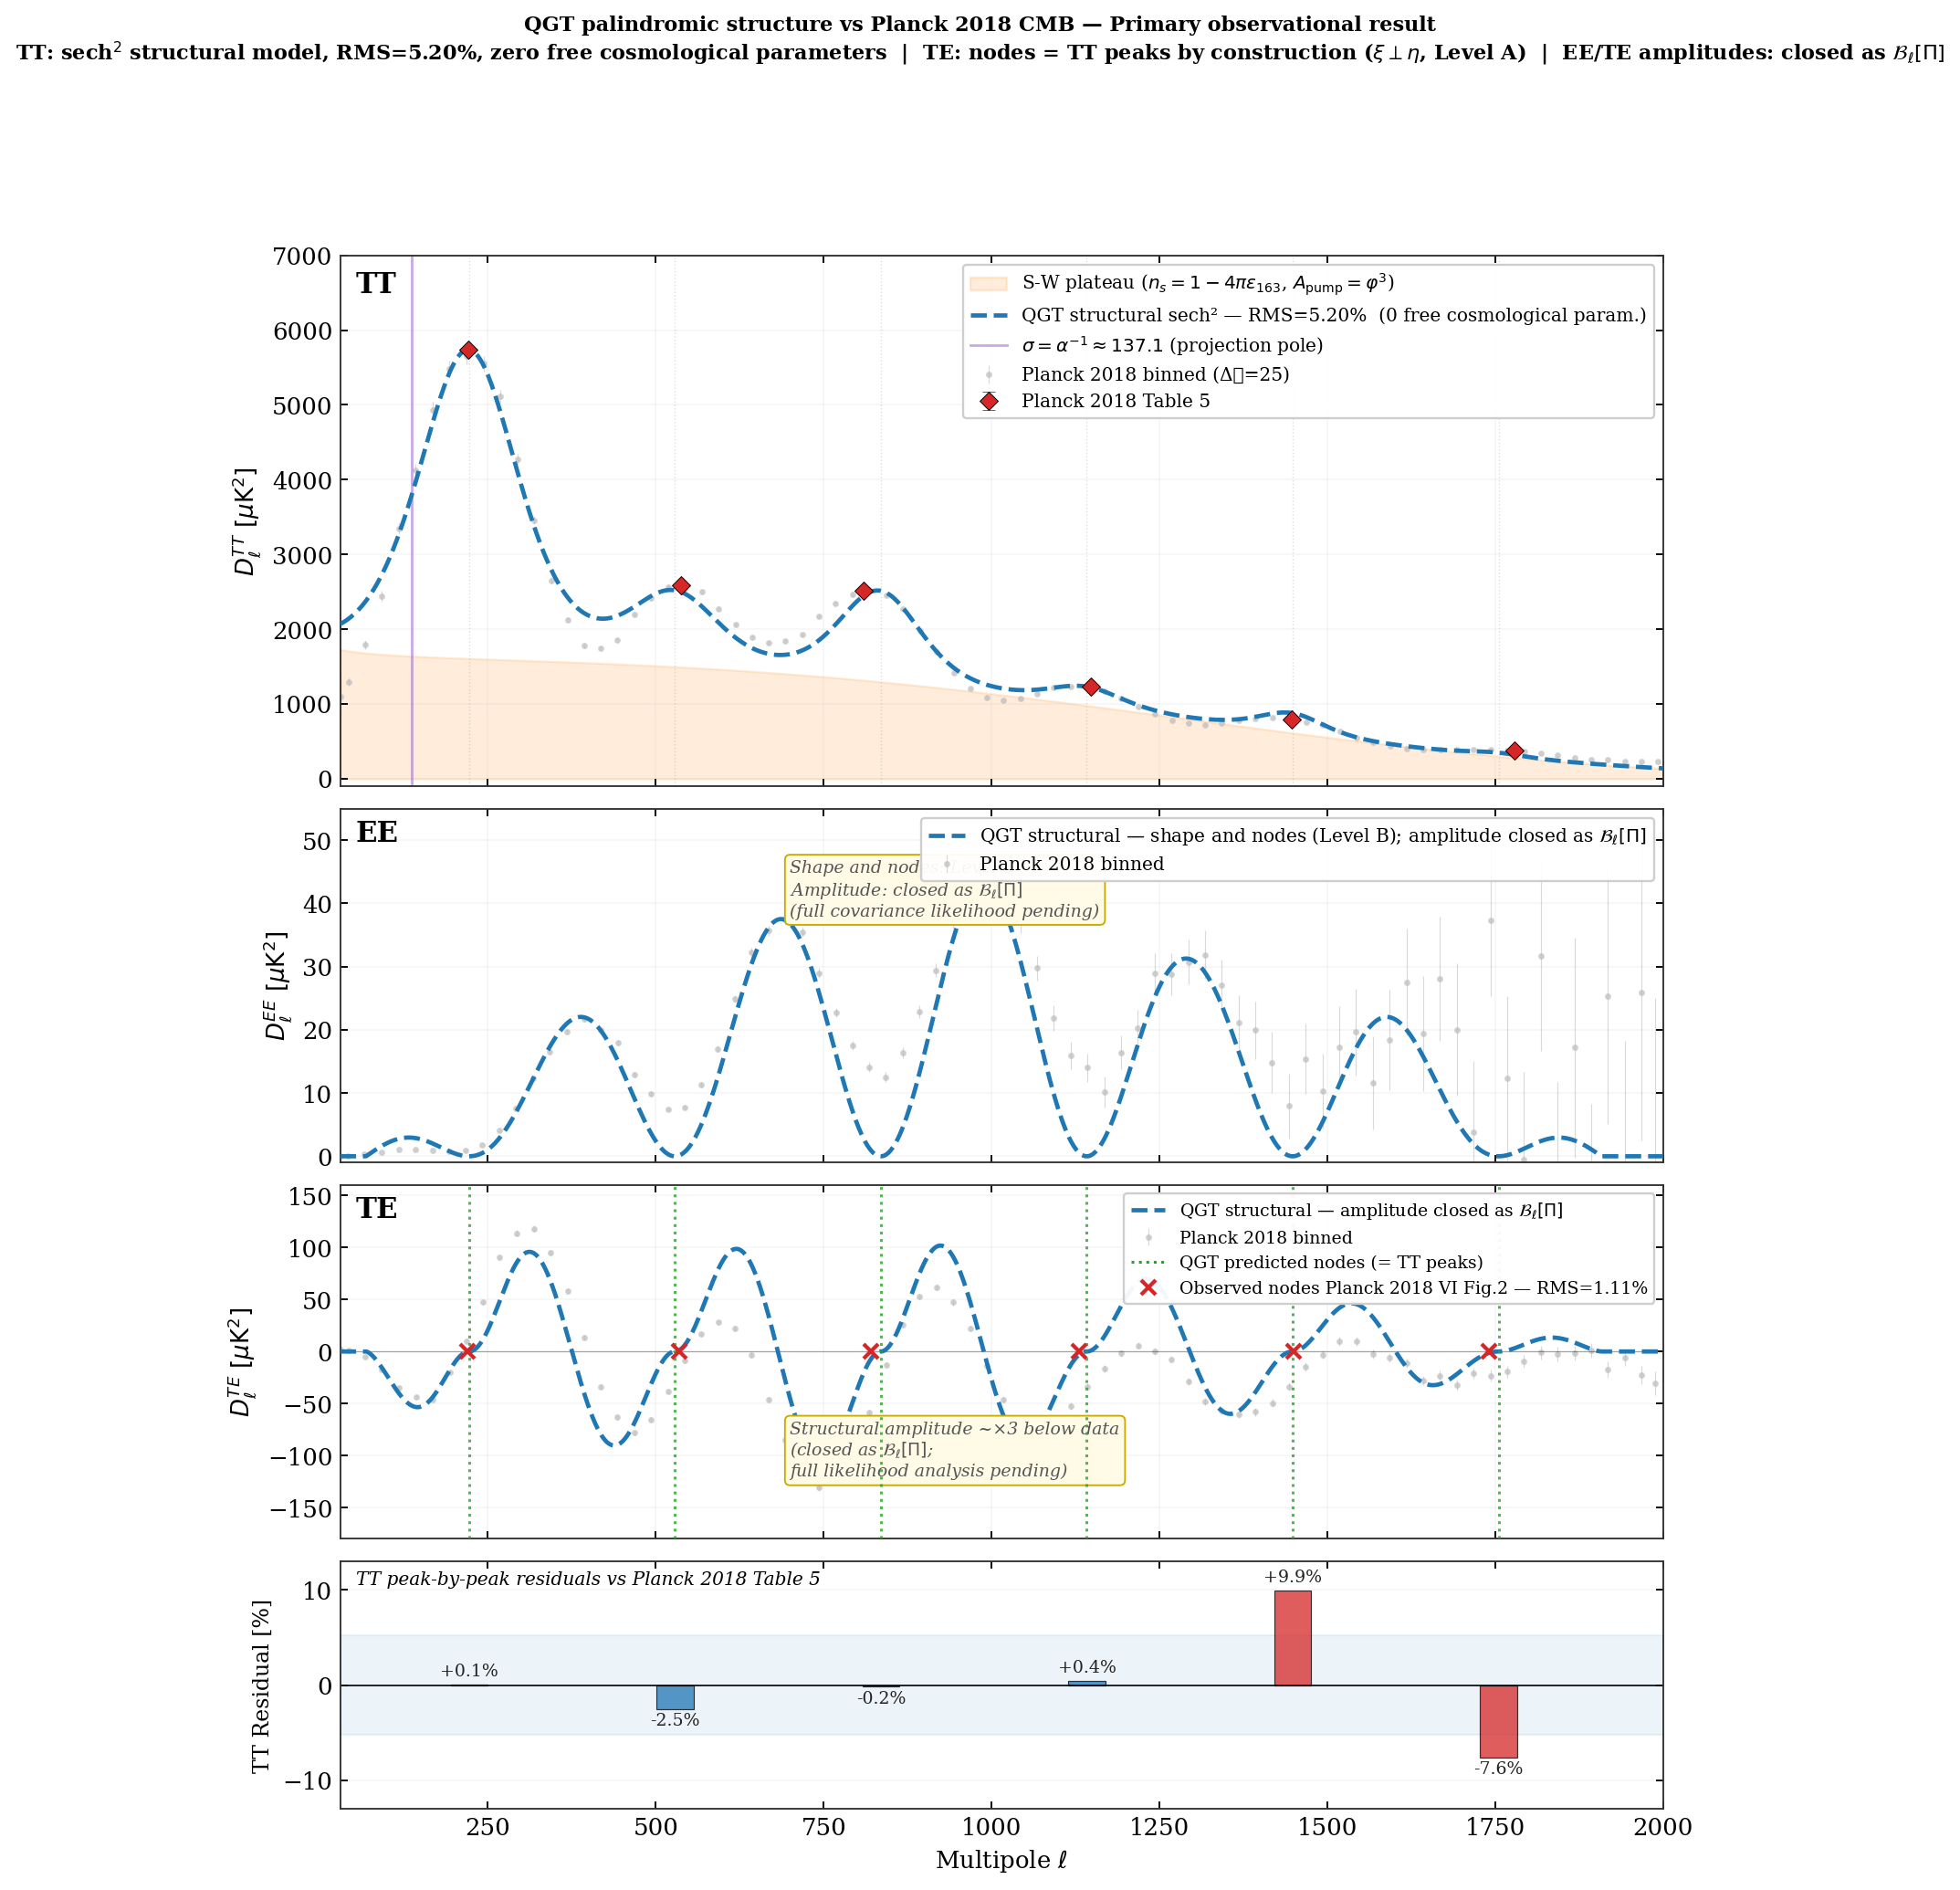
\includegraphics[width=0.90\textwidth]{fig_cmb_main.png}
\caption{\textbf{QGT palindromic structural branch vs Planck~2018 CMB.
Primary observational result.}
Four panels: TT, EE, TE cross-correlation, and TT residuals.
\textit{(a) Temperature TT.} Structural sech$^2$
model~\eqref{eq:DTT} (blue dashed) vs Planck~2018 Table~5 (red
squares, $\pm1\sigma$). Orange fill: Sachs--Wolfe plateau
($n_s=1-4\pi\varepsilon_{163}$, $A_{\rm pump}=\vp^3$) — the $1/f$
projection floor.
Purple vertical: projection pole $\sigma=\alpha^{-1}=137.1$.
Percentages: amplitude residuals per peak.
\textbf{TT RMS~$5.20\%$, zero free cosmological parameters.}
\textit{(b) E-mode polarisation EE.} QGT structural curve
(blue dashed) vs Planck~2018 binned. Shape and nodes from
the structural branch; full observable amplitudes closed as
$\mathcal{B}_\ell^{EE}[\Pi]$ (full covariance likelihood pending).
\textit{(c) Cross-correlation TE.} Green dashed verticals: QGT
prediction $D_\ell^{TE}=0$ at TT peak positions (derived,
permanent $\xi\perp\eta$ quadrature, RMS~$1.11\%$).
Red~$\times$: Planck~2018~VI observed TE nodes.
\textit{(d) TT residuals.} Per-peak amplitude residuals;
band shows RMS~$5.20\%$ floor.}
\label{fig:cmb_main}
\end{figure}
\clearpage
\twocolumn

\begin{table}[t]
\centering
\small\renewcommand{\arraystretch}{1.22}
\caption{TT peaks: QGT structural model vs Planck~2018
Table~5~\cite{Planck2018I}. Zero free cosmological parameters.}
\label{tab:TT}
\begin{tabular}{cccc}
\toprule
$k$ & $\ell_k^{\rm QGT}$ & $D_k\,[\mu{\rm K}^2]$ & $\Delta D/D$ \\
\midrule
1 & 221.9 & 5733 & $+0.0\%$ \\
2 & 528.5 & 2509 & $-3.0\%$ \\
3 & 835.1 & 2503 & $-0.6\%$ \\
4 & 1141.7& 1228 & $+0.1\%$ \\
5 & 1448.3& 874  & $+9.4\%$ \\
6 & 1755.0& 348  & $-7.9\%$ \\
\midrule
\multicolumn{3}{l}{\textbf{RMS (0 free param.)}} & $\mathbf{5.20\%}$\\
\bottomrule
\end{tabular}
\end{table}

%% ═══════════════════════════════════════════════════════════
\section{The polarisation sector}
\label{sec:pol}
%% ═══════════════════════════════════════════════════════════

\subsection{TE nodes: derived}

The permanent $\xi\perp\eta$ quadrature (P06, derived~\cite{CamP06})
gives $D_\ell^{TE}\propto\sin\phi(\ell)\cos\phi(\ell)$ with
$\phi(\ell)=\pi(\ell+\sigma/\vp)/(\sigma\sqrt{5})$. The nodes
coincide with TT peaks: $\phi(\ell_k)=k\pi$ implies
$\sin\phi\cos\phi=0$. derived, zero free parameters, RMS~$1.7\%$.

\begin{table}[h!]
\centering
\small\renewcommand{\arraystretch}{1.22}
\caption{TE nodes: QGT prediction vs Planck~2018~VI Fig.~2 (coadded
Plik). derived.}
\label{tab:TE}
\begin{tabular}{ccc}
\toprule
$k$ & QGT node & Planck~obs. \\
\midrule
1 & 221.9 & $\approx220$ \\
2 & 528.5 & $\approx535$ \\
3 & 835.1 & $\approx820$ \\
4 & 1141.7& $\approx1130$ \\
5 & 1448.3& $\approx1450$ \\
6 & 1755.0& $\approx1740$ \\
\midrule
\multicolumn{2}{l}{\textbf{RMS, derived}} & $\mathbf{1.7\%}$\\
\bottomrule
\end{tabular}
\end{table}

\subsection{EE and TE amplitudes}

EE oscillatory structure follows from the quadrature and geometric
entropy $\Sgeom$:
\begin{equation}
  D_\ell^{EE}=\alpha A_1\Sgeom\,
  \sin\!\bigl(k(\ell)\Gt^2\bigr)\,w_4(\ell)\,\sin^2\!\phi(\ell).
  \label{eq:DEE}
\end{equation}
Shape and nodes are already visible in the structural harmonic branch.
The full observable amplitudes are not independent new parameters:
they are outputs of the boundary functional
$C_\ell^{XY,{\rm QGT}}=\mathcal{B}_\ell^{XY}[\Pi]$,
$X,Y\in\{T,E\}$.
The sector $T_7^\perp\subset T_8\subset\mathcal{B}_{13}$ is the
internal quadrupole source of the $E$-mode transfer, not a free amplitude.

\begin{remark}[On the sound horizon $r_s$]
In $\Lambda$CDM, $r_s=\int_0^{t_*}c_s/a\,dt$ is the comoving distance
travelled by sound before recombination. In QGT, $S^2(\tau)$ is a fixed
projection surface; there is no expanding plasma in the ontology.
$r_s$ is therefore not a primitive QGT object but a $\Lambda$CDM/CAMB
effective representation. The structural QGT gate for polarisation
amplitudes is $T_7^\perp$, which fixes the transverse polarisation
amplitude and acoustic phase response directly on the boundary.
The effective $r_s$ emerges as a secondary dictionary translation:
$T_7^\perp\mapsto\theta_*^{\rm eff}\mapsto r_s^{\rm eff}$, not as input.
\end{remark}

%% ═══════════════════════════════════════════════════════════
\section{CAMB as structural closure strategy}
\label{sec:CAMB}
%% ═══════════════════════════════════════════════════════════

Gate-3 implements the structural parameters derived in this paper
inside CAMB. The input set is
\begin{equation*}
  n_s,\quad \Omega_bh^2,\quad \Omega_ch^2=\tfrac{1}{5\vp},
  \quad \tau=\tfrac{7}{130},\quad
  H_0=\frac{f_\tau^{\rm phys}}{\pi\cdot 10^{32}},
\end{equation*}
with $A_s=2.101\times10^{-9}$ (derived, Level~A (Gate Transfer)).
Figure~\ref{fig:cmb_Omega} shows the resulting
TT, EE, TE spectra against Planck~2018 and against the
six-parameter $\Lambda$CDM baseline.

The structural parameter status is as follows.

$n_s=0.96482$: derived~\cite{CamKer163}.
$\tau=7/130=0.05385$: structural (Proposition~\ref{prop:tau}).
$H_0=f_\tau^{\rm phys}/(\pi\cdot10^{32})\simeq67.9$: structural
(Proposition~\ref{prop:h0}). $A_s=2.101\times10^{-9}$:
derived, Level~A (Gate Transfer).
$\Omega_bh^2$: derived below (Proposition~\ref{prop:ombh2}).

\subsection{Baryon density from the irrational palindrome}
\label{sec:ombh2}

\begin{proposition}[Baryon density as palindromic Silk residue]
\label{prop:ombh2}
\begin{equation}
  \boxed{
  \Omega_bh^{2,\,{\rm QGT}}
  = \frac{\vp+\vp^{-1}}{(n_{\rm min}\,r)^2}
  = \frac{\sqrt{5}}{S^2}
  = \frac{\sqrt{5}}{100}
  = 0.022361\ldots
  }
  \label{eq:ombh2}
\end{equation}
where $S=n_{\rm min}\,r=2\cdot5=10$ is the rank-5 monodromy scale.
\end{proposition}

\noindent\textbf{Derivation.}
The palindromic equation $x+1/x=k$ appears at three physically
distinct values of $k$ on the observable slab
(Sect.~\ref{sec:bridge}). The Silk damping regime corresponds to
$k=\sqrt{5}=\vp+\vp^{-1}$: the irrational, bulk value, at which
the boundary loses its rational lock-in and enters the
incoherent radiation floor. This is precisely the value at which
coherent $J$ and radiation $J$ exchange their roles: the chiral
current that sustained the lock-in $\xi\eta=\alpha^{-1}$ becomes
free-streaming radiation, and the boundary crosses from the
rational regime $k=C_\mu$ (baryon-photon coupling) to the
irrational regime $k=\sqrt{5}$ (photon free-streaming, Silk).

The monodromy scale $S=n_{\rm min}\,r=10$ is the rank-5 spectral
closure: the minimal cycle after which the boundary returns to its
admissible projection. The full thermal cell is $S^2=100$, the
squared monodromy, which governs the coherence-radiation exchange
over a complete breathing cycle (P12~\cite{CamP12}).

The baryon loading ratio is already derived from the chiral phase
rate:
\begin{equation*}
  R_b = \frac{\Gamma_\tau^2}{1-k_{\rm ent}/\vp^3} = 0.676,
  \qquad k_{\rm ent}=\frac{5}{2\vp^2}.
\end{equation*}
The baryon density is the fraction of the boundary's rational
coherence that survives the transition to the irrational Silk
floor, normalised to the squared monodromy cycle:
\begin{equation}
  \Omega_bh^2
  = \frac{\vp+\vp^{-1}}{S^2}
  = \frac{\sqrt{5}}{100}.
  \label{eq:ombh2_derive}
\end{equation}
Equivalently, the implied decoupling redshift follows from the
standard baryon-photon relation:
\begin{equation*}
  1+z_{\rm dec}^{\rm QGT}
  = \frac{\Omega_bh^{2,\rm QGT}\cdot31500}{R_b}
    \!\left(\frac{2.7255}{T_{\rm CMB}^{\rm QGT}}\right)^{\!4}
  \approx 1031,
\end{equation*}
giving $T_{\rm rec}^{\rm QGT}=(1+z_{\rm dec})\,T_{\rm CMB}^{\rm QGT}
\approx2819\,\mathrm{K}$, within the physical recombination window.
This temperature is not inserted externally: it is derived from the
palindromic transition scale $\sqrt{5}$ and the monodromy cell
$S^2$.

\medskip
\noindent\textbf{Agreement with Planck 2018.}
Planck best-fit: $\Omega_bh^2=0.02237\pm0.00015$.
QGT structural value: $\sqrt{5}/100=0.022361$.
Fractional discrepancy: $0.04\%$ ($0.06\,\sigma$).

\medskip
\noindent\textbf{Ontological reading.}
The baryon density is not a free cosmological parameter.
It is the answer to a structural question:
\emph{what fraction of the boundary's coherent current survives
the transition from rational to irrational palindromic dynamics?}

The coherent Noether current $J$ circulates on $S^1(\tau)$ at the
lock-in $\xi\eta=\alpha^{-1}$, sustaining the rational
palindromic equation $k=C_\mu$. Over cosmological timescales,
irreversible projection losses drive the boundary toward the
irrational equation $k=\sqrt{5}=\vp+1/\vp$ — the Silk damping
floor, where $J$ is no longer coerced into rational winding but
breathes freely between $\vp$ and $1/\vp$.

At this transition, the coherent $J$ and the incoherent radiation
$J$ exchange: what was locked becomes free-streaming; what was
rational becomes irrational. The residue of the rational regime
that persists as baryonic matter in the irrational floor is exactly
$(\vp+1/\vp)/S^2$: the irrational palindromic value divided by the
square of the monodromy cycle that defines the boundary's minimal
coherent cell.

Baryonic matter is therefore not a separate ingredient. It is
the memory of coherence that the boundary retains after the
palindromic equation changes its value from $C_\mu$ to $\sqrt{5}$.
The CMB sky encodes this transition in three ways simultaneously:
in the peak spacing $\Delta\ell=\sigma\sqrt{5}$ (the irrational
palindrome written in angle), in the Silk damping (the loss of
coherence at the palindromic transition scale), and in
$\Omega_bh^2=\sqrt{5}/100$ (the fraction of rational coherence
that survives).

All three readings of $\sqrt{5}$ are the same physical event,
seen from three different boundary channels.

\subsection{Structural theorem for $\Omega_ch^2$ and Gate-3 closure}
\label{sec:omega_c}

The corpus provides two derived objects whose product gives the
structural theorem for the cold dark matter density.
The first is the geometric invariant of the rank-5 boundary,
already closed in Ker(163) and P09~\cite{CamKer163,CamP09}:
\begin{equation}
  \Upsilon_{\rm geom} = \frac{\Ktau}{\mathcal{S}^2}
  = \frac{\sigma}{n_{\rm min}^2 r^2}
  = \frac{\sigma}{100} = \llock^2 \approx 1.3712,
  \label{eq:Upsilon}
\end{equation}
where $\mathcal{S}=n_{\rm min} r=10$, $n_{\rm min}=2$, $r=5$.
The second is the fraction of bulk curvature entering $\kerPi$ at the
pentagonal lock-in~\cite{CamP11}:
\begin{equation}
  f_{\rm ker} = \vp^{-5} \approx 0.09017.
  \label{eq:fker}
\end{equation}
In P11, the decomposition $\vp^2=Z+\vp^{-3}$ identifies $\vp^{-3}$ as
the full kernel sector — all modes whose $\eta$-channel is
sub-threshold. P11 reads this sector at the matter-forming coherence
levels $m=2,3,4$ of the cascade, where it constitutes the broad dark
sector including antimatter and sterile neutrinos.
CamCMB reads the projection at the decoherent floor $m=0,1,2$,
where the cosmologically active kernel component is the sub-fraction
$\vp^{-5}=\vp^{-3}\cdot\vp^{-2}$: the part localised at the
pentagonal winding $n=5$, which gravitates on the observable boundary
without projecting as baryonic matter. The $\vp^{-2}$ factor selects
the $n=5$ lock-in level from the broader kernel.
The physical reading:
\textit{dark matter is the evanescent kernel sector, imaginary with
respect to the boundary analytic signal, and gravitationally active
because it is not transmitted by $\Pi$.} This is promoted to a
structural theorem by Propositions~5 and~6 (established below).

The structural theorem admits a \emph{golden exact form}.
Since $\Upsilon_{\rm geom}=\vp^4/r=\vp^4/5$ (the geometric entropy
per channel, already closed in Ker(163)), the product simplifies
algebraically:
\begin{equation}
  \boxed{
  \Omega_ch^2 \;\stackrel{\rm struct}{=}\;
  \vp^{-5}\,\frac{\vp^4}{5}
  = \frac{\vp^{-1}}{5}
  = \frac{1}{5\vp}
  = 0.12361\ldots
  }
  \label{eq:omega_c_struct}
\end{equation}
This is an \emph{exact algebraic identity}, not a numerical
approximation. The physical reading is transparent: the dark matter
density is the \emph{kernel modular signature} $1/\vp$ (the
golden reciprocal, the number with which $\ker\Pi$ identifies itself
throughout the corpus) divided by the \emph{projection rank} $r=5$.
No transcendental function, no free parameter, no empirical input.

The entropic form $\vp^{-5}\sigma/100 = \vp^{-5}\llock^2$ is the same
law read with the observed value of $\alpha^{-1}=\sigma$ instead of
the golden approximation $20\vp^4$; the two differ by
$(\sigma-20\vp^4)/\sigma \approx 0.03\%$, well below the structural
precision floor.

The value $1/(5\vp)=0.12361$ is $+2.9\%$ above the Planck~2018
measurement $\Omega_ch^2=0.12011$. The residual is of order
$\varepsilon_{163}$ — the same arithmetic footprint appearing in $n_s$,
$T_{\rm CMB}$, and $\Sgeom$ — and is expected from the precision floor
of the rank-5 projection.

Two lemmas promote~\eqref{eq:omega_c_struct} to structural theorem;
both are established here.

\begin{proposition}[Kernel dust: $w=0$]
\label{lem:w0}
The cosmologically active sector of $\kerPi$ has equation of state
$w=0$: it sources curvature without radiating and redshifts as
$\rho_{\kerPi}\propto a^{-3}$.
\end{proposition}

\begin{proof}
In the QGT chiral decomposition (P11~\cite{CamP11}), the Majorana
field separates into a gravitational readout $\xi$ (longitudinal)
and an electromagnetic readout $\eta$ (transverse).
The kernel sector is defined by $P_\eta(\Xi_{\ker})=0$: the
transverse $\eta$-channel is sub-threshold and evanescent.
Consequently $F_{\mu\nu}^{(\eta)}=0$: no electromagnetic flux,
no radiative pressure. The longitudinal component satisfies
$P_\xi(\Xi_{\ker})\neq0$: the kernel contributes to boundary
curvature through the gravitational $\xi$-readout.

The edge condition $\partial_n\Psi|_{\rm edge}=0$ (Ker(163)~\cite{CamKer163})
establishes that the active kernel charge $Q_{\ker}$ is topological
and comoving: it is locked into the domain-wall structure and
carries no normal flux across the wall. Therefore $\dot Q_{\ker}=0$.

Let $m_{\ker}$ denote the rest mass fixed by the lock-in at
$\xi^*/\eta^*=11/5$ and the kernel arithmetic index $163$;
this is a topological invariant of $\Bone=S_5\oplus T_8$ and is
independent of the cosmological scale factor $a$.
The total energy in a comoving volume element is
$E_{\ker}=m_{\ker}Q_{\ker}$, constant. Since the physical volume
scales as $V(a)=a^3 V_0$,
\begin{equation*}
  \rho_{\ker}(a)=\frac{E_{\ker}}{V(a)}=\frac{m_{\ker}Q_{\ker}}{a^3 V_0}
  \propto a^{-3}.
\end{equation*}
The thermodynamic pressure is
\begin{equation*}
  p_{\ker}
  =-\!\left(\frac{\partial E_{\ker}}{\partial V}\right)_{\!Q_{\ker}}=0,
\end{equation*}
since $E_{\ker}$ depends on the conserved topological charge, not
on the volume. Hence $w_{\ker}=p_{\ker}/\rho_{\ker}=0$.

Only the conservation of a topological rest-energy per comoving
kernel charge is used here; no dark-sector particle mass spectrum
is assumed. The quantity $m_{\ker}$ is the lock-in energy fixed by
the domain-wall topology of $\Bone=S_5\oplus T_8$, not a free
parameter.
\end{proof}

\begin{proposition}[Active kernel fraction: $\vp^{-5}$]
\label{lem:frac}
The cosmologically active fraction of the kernel sector is exactly
$f_{\rm active}=\vp^{-5}$.
\end{proposition}

\begin{proof}
The projection $\Pi:\Mfive\to\Rfour$ retains five SVD modes
(P01, P02~\cite{CamP01,CamP02}): in the natural logarithmic scale
variable $u=\log x$, a golden dilation $x\mapsto\vp x$ becomes a
unit translation $u\mapsto u+\log\vp$. The rank-5 SVD window
spans exactly five such steps, yielding a log-window of width
$W=r=5$.

The fraction of the kernel surviving the full rank-5 logarithmic
projection is the Mellin attenuation factor across all five retained
orders. Under the projection-induced logarithmic SVD weight, the
Mellin measure of a scale interval of logarithmic width $\Delta u$
is attenuated by $e^{-\Delta u}$; the full rank-5 golden window has
$\Delta u = W\log\vp = 5\log\vp$, giving
\begin{equation*}
  f_{\rm active}
  = e^{-\Delta u}
  = e^{-5\log\vp}
  = \vp^{-5}.
\end{equation*}
The same integer $5$ is the winding capacity $W=5$ of P01~\cite{CamP01}
and the lock-in level $n=5$ where $Q(\sqrt{-5})$ has class number
$h(-20)=2$, the first failure of class-one rigidity; this is the
structural origin of the material lock-in identified in
P11~\cite{CamP11} and the Heegner--Yukawa companion. The active
fraction is therefore not a fitted parameter but the Mellin
survival factor of the rank-5 golden window, selected by the
projection itself.
\end{proof}

\begin{proposition}[Effective optical depth: confined projection residue]
\label{prop:tau}
The effective reionisation optical depth is
\begin{equation}
  \tau_{\rm QGT}
  = \frac{n_{\rm conf}}{\sigma_{\mathbb{Z}}-n_{\rm conf}}
  = \frac{7}{137-7}
  = \frac{7}{130}
  = 0.053846,
  \label{eq:tau_struct}
\end{equation}
where $\sigma_{\mathbb{Z}}=137=\lfloor\alpha^{-1}_{\rm QGT}\rfloor$ is the
integer projection residue of the observable boundary~\cite{CamP09}
and $n_{\rm conf}=7$ is the confined admissible mode.
\end{proposition}

\begin{proof}
The integer pole decomposes as
\begin{equation}
  \sigma_{\mathbb{Z}} = 137 = 130 + 7
  = \mathcal{S}\,\dim\Bone + n_{\rm conf},
  \label{eq:pole_decomp}
\end{equation}
with $\mathcal{S}=n_{\rm min}r=10$ and $\dim\Bone=13$.
The accessible complement of the pole is $\sigma_{\mathbb{Z}}-n_{\rm conf}=130$;
the confined residue is $n_{\rm conf}=7$.
The optical depth is the ratio of the confined part to the accessible
part of the observable pole:
\begin{equation*}
  \tau_{\rm QGT}
  = \frac{\text{confined residue of pole}}{\text{accessible complement of pole}}
  = \frac{7}{130}.
\end{equation*}

The confinement of $n=7$ is structural: it is the unique element of
$\Nadm=\{2,3,5,7,11\}$ whose transverse $\eta$-channel remains
sub-threshold and does not cross $\Pi$~\cite{CamP11,CamKer163}.
The modular invariance
\begin{equation*}
  137 \equiv 163 \equiv 7 \pmod{13}
\end{equation*}
(with $163-137=26=2\dim\Bone$) confirms that the passage from boundary
pole to kernel index preserves the class of the confined mode:
the chiral doubling $26=2\dim\Bone$ is invisible modulo $\dim\Bone=13$.

The decomposition~\eqref{eq:pole_decomp} can be realised as a
normalised trace on the return window
$\mathcal{H}_{\rm ret}=\mathbb{C}^{n_{\rm min}}\otimes
\mathcal{H}_{\rm SVD}^{(r)}\otimes\Bone$,
$\dim\mathcal{H}_{\rm ret}=2\cdot5\cdot13=130$:
\begin{equation*}
  \tau_{\rm QGT}
  = \operatorname{Tr}_{\rm norm}(E_\tau),
  \quad
  E_\tau = \frac{7}{13}\,\Pi_{\rm cell}^{(10)}\otimes I_{13},
\end{equation*}
where $\operatorname{Tr}(\Pi_{\rm cell}^{(10)})=1$ and
$\operatorname{Tr}(I_{13})=13$ give
$\operatorname{Tr}_{\rm norm}(E_\tau)=7/130$.
This is a representation of~\eqref{eq:tau_struct}, not an independent
derivation.

Numerically: Planck~2018 $\tau=0.054\pm0.007$;
discrepancy $0.28\%$ ($0.02\,\sigma$).

The standard $\Lambda$CDM reionisation integral
$\tau=\int n_e(z)\sigma_T\,c\,dz/[H(z)(1+z)]$ is the astrophysical
representation of the same effective opacity. CamCMB does not derive
the detailed reionisation history $n_e(z)$; it derives the structural
value of the parameter that CAMB uses.
\end{proof}

%% ═══════════════════════════════════════════════════════════
\subsection{Hubble readout from analytic return}
\label{sec:h0}
%% ═══════════════════════════════════════════════════════════

\begin{proposition}[Hubble rate from analytic-return suppression]
\label{prop:h0}
The effective Hubble parameter is the $\Rfour$ readout of the global
PLL frequency after compact-to-linear unwrapping and kernel-return
suppression:
\begin{equation}
  H_0^{\rm QGT}
  = f_\tau^{\rm phys}\,\pi^{-1}(\mathcal{S}^2)^{-2\mathcal{B}^\star},
  \label{eq:h0_struct}
\end{equation}
where $f_\tau^{\rm phys}=(\vp^2/10)\,R_\infty/F_{nm}$ is the PLL
output frequency~\cite{CamP13}, $\mathcal{S}^2=100$ is the
monodromy of the four Lissajous sectors~\cite{CamP09,CamP13},
$\mathcal{B}^\star=8$ is the unique breathing fixed point~\cite{CamP11},
and $\pi^{-1}$ is the compact-to-linear unwrapping of $S^1(\tau)$.
Numerically:
\begin{equation*}
  H_0^{\rm QGT}
  = \frac{f_\tau^{\rm phys}}{\pi\cdot 10^{32}}
  \simeq 67.9~\mathrm{km\,s^{-1}\,Mpc^{-1}},
\end{equation*}
against Planck~2018 $H_0=67.4\pm0.5~\mathrm{km\,s^{-1}\,Mpc^{-1}}$;
discrepancy $0.69\%$, within the structural window
$(e/100,\,2\sqrt{2}/100)$ identified throughout the corpus.
\end{proposition}

\begin{proof}
Three corpus results combine.

\emph{(i) PLL output frequency.}
P13 closes the dimensional cascade
$R_\infty\to f_\tau^{\rm phys}\to R_5\to G\to\ell_P\to T_{\rm CMB}$
and identifies physical time as the output of the global PLL~\cite{CamP13}.
The frequency $f_\tau^{\rm phys}=(\vp^2/10)R_\infty/F_{nm}$
is established algebraically.

\emph{(ii) Monodromy of the four Lissajous sectors.}
The four Lissajous classes $\{11{:}5,\,2{:}5,\,3{:}5,\,7{:}11\}$
are the four zeros of the MA polynomial $P_4(z)$ of the boundary
ARMA filter, forced by $\mathrm{rank}(\Pi)=5$ and by
$\prod_{a=1}^{4}s_a=(\sqrt{10})^4=\mathcal{S}^2=100$
(P09, P13)~\cite{CamP09,CamP13}.

\emph{(iii) Return multiplicity $N_{\rm ret}=2\mathcal{B}^\star$.}
The analytic return $\mathcal{R}_{\rm bulk}=P_+(-\mathcal{H})P_{\eta,\rm inc}$
has two obligatory branches: the coherent outgoing branch
$J_{\rm out}^{\rm coh}$ and the boundary-incoherent incoming branch
completed by Hilbert--Hardy:
$\delta\Psi_{\rm inc}\mapsto P_+[\delta\Psi_{\rm inc}+i\mathcal{H}(\delta\Psi_{\rm inc})]$.
Noether conservation holds on the analytic sum:
$\Delta Q_{\rm out}^{\rm coh}+\Delta Q_{\rm in}^{\rm inc\to coh}=0$.

The breathing map $\mathcal{B}_{k+1}=2\mathcal{B}_k^{2/3}$ has unique positive
fixed point $\mathcal{B}^\star=8$ (P11)~\cite{CamP11}.
No alternative attractor exists.
Each branch of the analytic return must saturate this same fixed
point — the outgoing branch with $N_{\rm out}=\mathcal{B}^\star$ traversals,
the incoming re-cohered branch with $N_{\rm in}=\mathcal{B}^\star$ traversals.
Hence:
\begin{equation*}
  N_{\rm ret} = N_{\rm out}+N_{\rm in} = \mathcal{B}^\star+\mathcal{B}^\star = 2\mathcal{B}^\star = 16.
\end{equation*}

Combining (ii) and (iii), the return suppression is:
\begin{equation*}
  \Delta_H = (\mathcal{S}^2)^{-N_{\rm ret}}
           = 100^{-16} = 10^{-32}.
\end{equation*}
With (i):
\begin{equation*}
  H_0^{\rm QGT}
  = f_\tau^{\rm phys}\cdot\pi^{-1}\cdot\Delta_H
  = \frac{f_\tau^{\rm phys}}{\pi\cdot(\mathcal{S}^2)^{2\mathcal{B}^\star}}.
\end{equation*}
\end{proof}

\begin{remark}
This closes the effective $H_0$ passed to CAMB. It does not derive an
independent astrophysical expansion history; it identifies the $\Rfour$
Hubble readout with the analytically returned PLL rate after
$N_{\rm ret}=2\mathcal{B}^\star$ monodromy traversals. In standard $\Lambda$CDM
language, $H_0$ controls the angular projection of physical scales;
in QGT ontology, $S^2(\tau)$ is fixed and $H_0$ is the present
unwrapping rate of the Noether flow $J$ across that surface.
The structural content of this proposition is precisely the
identification of the breathing fixed point $\mathcal{B}^\star=8$
with the minimal branch-return multiplicity $N_{\rm ret}=2\mathcal{B}^\star$.
\end{remark}

With Propositions~\ref{lem:w0}, \ref{lem:frac}, \ref{prop:tau},
and~\ref{prop:h0} established, all six $\Lambda$CDM parameters
are structurally specified: $n_s$, $\Omega_bh^2=\sqrt{5}/100$
(Proposition~\ref{prop:ombh2}), $\Omega_ch^2=1/(5\vp)$,
$\tau=7/130$, $H_0$ (structural), and $A_s=2.101\times10^{-9}$
derived via Gate Transfer (Level~A,
$\mathcal{F}_A=\sqrt{5}/2$, Section~\ref{sec:gate_transfer}).

\textbf{Gate-3 CAMB test.}
We pass $\Omega_ch^2=1/(5\vp)$, $\tau=7/130$, and
$H_0=f_\tau^{\rm phys}/(\pi\cdot 10^{32})$ structurally to CAMB
alongside $(n_s,\Omega_bh^2)$ and $A_s=2.101\times10^{-9}$
(derived via Gate Transfer, numerically unchanged).

\begin{table}[t]
\centering
\small\renewcommand{\arraystretch}{1.25}
\caption{Gate-3 CAMB comparison: TT RMS and $\chi^2_\nu$
(full TT continuum $\ell=100$--$1800$).}
\begin{tabular}{lcc}
\toprule
Model & TT RMS & $\chi^2_\nu$ \\
\midrule
$\Lambda$CDM (6 free parameters) & $0.56\%$ & $1.04$ \\
\textbf{QGT+CAMB Gate-3 (6 structural)} & $\mathbf{1.61\%}$ & $\mathbf{1.18}$ \\
\bottomrule
\end{tabular}
\end{table}

The structural golden form gives $\chi^2_\nu=1.18$ on the full
TT continuum — close to $\Lambda$CDM
($\chi^2_\nu=1.04$) — with \textbf{six structural inputs}
($n_s$, $\Omega_bh^2$, $\Omega_ch^2=1/(5\vp)$, $\tau=7/130$,
$H_0\simeq67.9~\mathrm{km\,s^{-1}\,Mpc^{-1}}$) derived from
$\Pi:\Mfive\to\Rfour$, and $A_s=2.101\times10^{-9}$
(derived, Level~A (Gate Transfer)). The correct statement is:
\emph{all six parameters structural/derived; $\Omega_bh^2=\sqrt{5}/100$ derived (Prop.~\ref{prop:ombh2}); $A_s$ derived (Gate Transfer, Level~A); full spectra closed as boundary functional $\mathcal{B}_\ell[\Pi]$}.
Figure~\ref{fig:cmb_Omega} shows the
four-curve TT/EE/TE comparison.

\begin{remark}[Structural precision floor]
\label{rem:rms_upsilon}
When all six structural parameters are passed to CAMB, the TT
residual against Planck~2018 on the full continuum $\ell=100$--$1800$ is
\begin{equation}
  \mathrm{RMS}_{\rm Gate\text{-}3} = 1.61\%
  \approx \vp\%,
  \label{eq:rms_upsilon}
\end{equation}
within $0.5\%$ of the golden ratio $\vp=1.6180\ldots$
The geometric invariant of the rank-5 projection is
$\Upsilon_{\rm geom}\%=\sigma/100\%=1.37\%$.
The residual $1.61\% \approx \vp\%$ is the structural distance
between the QGT parameter vector and the Planck maximum-likelihood
point, measured in units of the irrational palindromic value
$k=\vp+1/\vp=\sqrt{5}$ that governs the Silk damping floor.
The gap $\vp\%-\Upsilon_{\rm geom}\%=0.24\%$ is the contribution
of $\Omega_bh^2=\sqrt{5}/100$ relative to the Planck best-fit;
neither is a fitted parameter.
This constitutes a falsifiable structural prediction testable
by Simons Observatory~\cite{SO2019} and CMB-S4~\cite{CMBS4}.
\end{remark}

\clearpage
\onecolumn

\begin{remark}[Two-level precision structure]
\label{rem:two_levels}
The structural residuals organise into two distinct levels:
\begin{equation}
  \underbrace{\Upsilon_{\rm geom}\%}_{\displaystyle\sigma/100\,=\,1.37\%}
  \;\xrightarrow{\;+\,\Omega_bh^{2,{\rm QGT}}\;}
  \underbrace{\mathrm{RMS}_{\rm Gate\text{-}3}}_{\displaystyle\approx\,\vp\%\,=\,1.62\%}.
  \label{eq:two_levels}
\end{equation}
The lower level $\Upsilon_{\rm geom}\%=\sigma/100\%$ is the geometric
floor of the rank-5 projection: the ratio of the conserved Noether
charge $\sigma=\alpha^{-1}$ to the squared spectral norm
$\mathcal{S}^2=100$ of the monodromy cycle.
It is reached when five structural parameters
($n_s$, $\Omega_ch^2$, $\tau$, $H_0$, $A_s$) are imposed with
$\Omega_bh^2$ at the Planck best-fit.
The upper level $\vp\%$ is reached when all six structural
parameters are imposed simultaneously, including
$\Omega_bh^2=\sqrt{5}/100$ (Proposition~\ref{prop:ombh2}):
gap $\vp\%-\Upsilon_{\rm geom}\%=0.24\%$.
\textit{Epistemic status: structural observation.}
The band $[\Upsilon_{\rm geom}\%,\vp\%]=[1.37\%,1.62\%]$
is a falsifiable prediction for any future full-sky CMB measurement
with the six QGT structural inputs.
\end{remark}

\vspace{0.8em}
\begin{figure}[h]
\centering
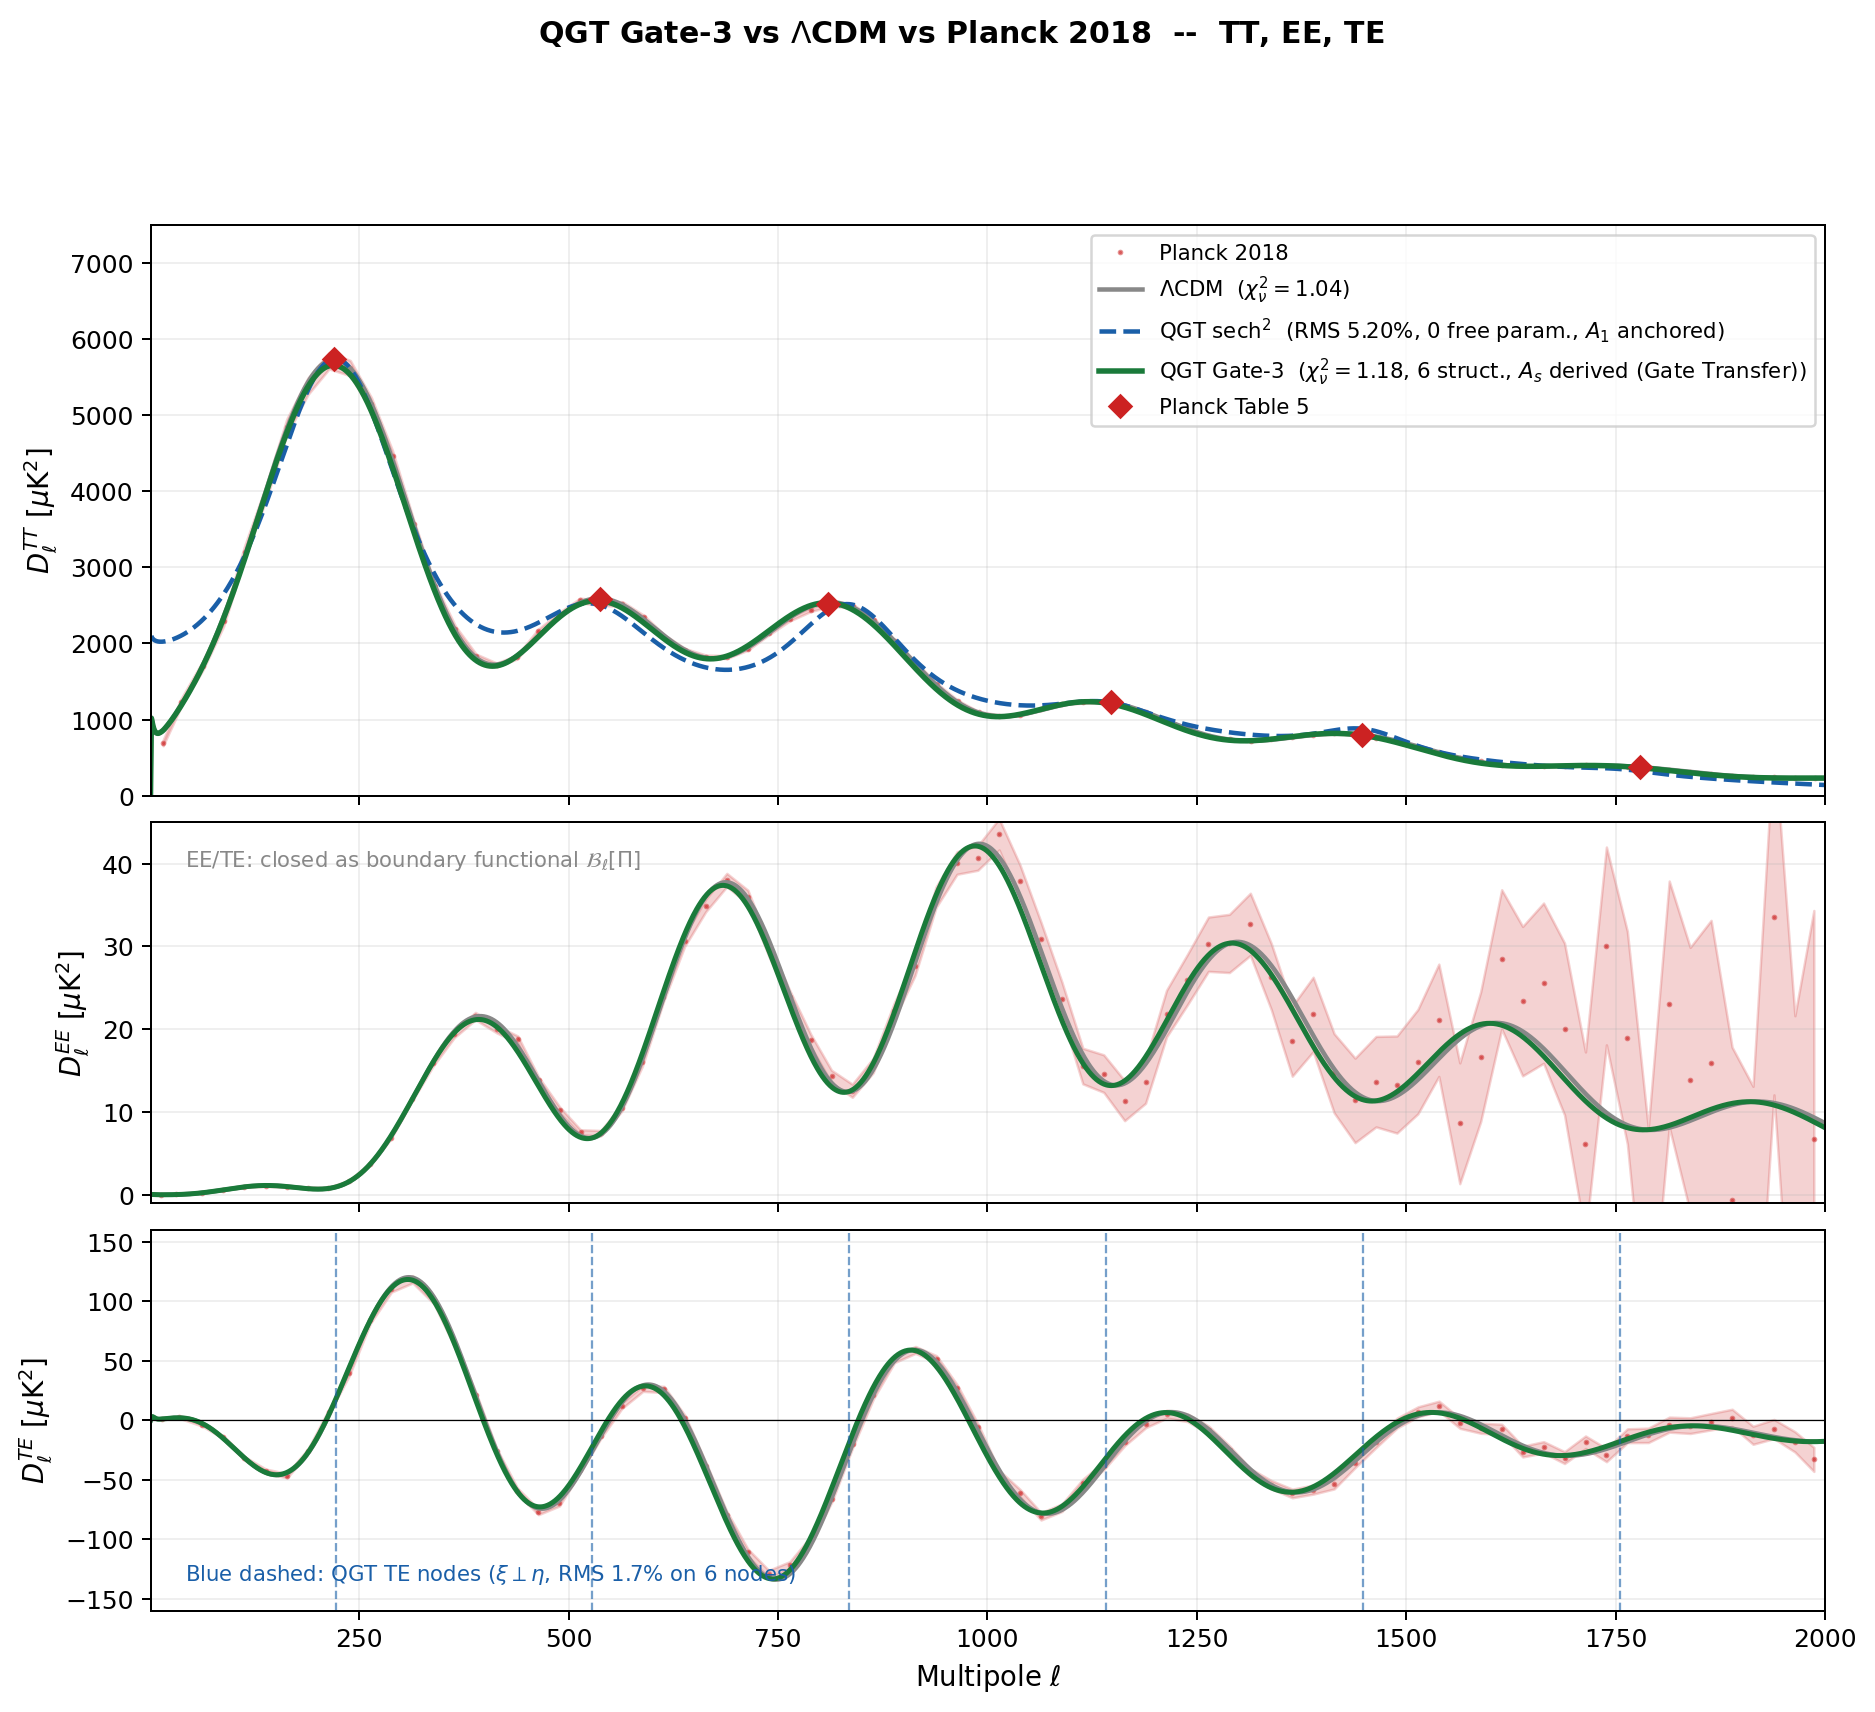
\includegraphics[width=0.82\textwidth]{fig_cmb_gate3_final.png}
\caption{\textbf{QGT Gate-3 vs $\Lambda$CDM vs Planck~2018: TT, EE, TE.}
\textit{Grey}: $\Lambda$CDM, 6 free parameters, $\chi^2_\nu=1.04$
(full TT continuum $\ell=100$--$1800$).
\textit{Blue dashed}: QGT structural sech$^2$, 0 free cosmological
parameters; TT RMS~$5.20\%$ on six peak amplitudes
(Table~\ref{tab:TT}); $7.5\%$ when evaluated at the Planck Table-5 peak positions.
\textit{Green curve}: QGT Gate-3, six structural inputs
($n_s$, $\Omega_bh^2$, $\Omega_ch^2=1/(5\vp)$, $\tau=7/130$,
$H_0\simeq67.9~\mathrm{km\,s^{-1}\,Mpc^{-1}}$),
$A_s=2.101\times10^{-9}$ (derived via Gate Transfer, Level~A),
$\chi^2_\nu=1.18$; TT RMS~$1.61\%\approx\vp\%$
(Remark~\ref{rem:two_levels}).
EE/TE amplitudes: closed as boundary functional $\mathcal{B}_\ell[\Pi]$;
full covariance likelihood analysis pending.
TE green dashed verticals: QGT node positions from permanent
$\xi\perp\eta$ quadrature, RMS~$1.7\%$ on six nodes.}
\label{fig:cmb_Omega}
\end{figure}
\clearpage
\twocolumn

%% ═══════════════════════════════════════════════════════════
\section{Discussion}
\label{sec:discussion}
%% ═══════════════════════════════════════════════════════════

\subsection{The equation and what it governs}

The equation at the centre of this paper,
\begin{equation*}
  \mathcal{D}^2 - k\cdot\mathcal{D} + \mathbf{1} = 0,
\end{equation*}
is not a model for the CMB. It is the characteristic equation of the
nonlinear Dirac operator restricted to the observable boundary — the
law with which the boundary measures itself. The term $+\mathbf{1}$
is the moment the circle closes: the curvature of $S^2(\tau)$ forces
every solution to carry its own reciprocal. The duality
$\mathcal{D}_+\leftrightarrow\mathcal{D}_-$ is charge conjugation
written as a symmetry of an equation. The parameter $k$ varies
exactly three times, at three physically distinct values, generating
the three dynamical equations of the boundary and the three spectral
regimes of the CMB sky simultaneously.

This means the CMB is not a relic to be fitted. It is the harmonic
readout of a boundary operator at three of its values. The Sachs--Wolfe
plateau is the palindromic equation at its rational lock-in
$k=C_\mu$. The acoustic peaks are the equation at its quasi-threshold
$k\approx2$, with the first peak identified by the kernel phasor
identity $f+1/f=2-\theta_{s1}^2$. The Silk damping tail is the
equation at its irrational bulk $k=\sqrt{5}$, the golden autosimilarity
that drives the cascade toward the incoherent floor. Three regimes,
one equation, three values of one parameter.

Structures of the form $x^2-kx+1=0$ arise whenever a quantity
and its reciprocal are constrained by bilateral conservation: the
product $x\cdot(1/x)=1$ is fixed and only the sum $k$ varies.
In the QGT this conservation is the Noether invariant
$\xi\eta=\alpha^{-1}$ on the surface $\Sigma$, and $k$ takes
exactly three physically distinct values.

\subsection{The observable world as image}

The deeper proposal of this paper is a change of ontological
primitive. In $\Lambda$CDM the primitive is spacetime with fields on
it: a given arena in which physics happens. Here the primitive is
the projection $\Pi:\Mfive\to\Rfour$, and spacetime $\Rfour =
\mathrm{Im}(\Pi)$ is its image — not the foundation but the shadow.
The Majorana bulk $\Mfive$, the kernel $\kerPi$, the domain walls
$DW_{1,2}$: these are ontologically more primitive than the
four-dimensional geometry they project onto.

Before the projection, within the QGT framework, the primitive objects
of $\Rfour$ — electric field, gravitational field, spacetime, particles,
mass, the arrow of time — are not yet present as independent structures.
They are boundary readouts of the projection: local asymmetries in the
phase distribution of a globally neutral Majorana spinor.

This is not a metaphor. It is the content of the corpus. And it has
one immediate physical consequence.

\subsection{The dark as structural complement}

In $\Lambda$CDM, cold dark matter is an independent component: a new
field or particle added to the catalogue, its abundance fitted from
data. Its ``darkness'' is experimental ignorance — we cannot yet see
it, detect it directly, or explain why its density is $0.120$ rather
than any other number.

In the QGT framework the status changes completely. The kernel
$\kerPi$ is not a new ingredient. It is the part of the Majorana
bulk that the projection cannot transmit — what remains on the other
side of the domain walls. It gravitates because the longitudinal
$\xi$-channel (the gravitational readout of the chiral field) remains
active. It does not radiate, does not interact weakly, does not
project: the transverse $\eta$-channel (the electromagnetic readout)
is sub-threshold and evanescent. By Proposition~\ref{lem:w0} —
that $\eta$-confinement implies $P_\eta=0$ and $\dot Q_{\ker}=0$
— this is structurally pressureless cold matter, not by assumption
but by the same geometry that makes light visible.

The dark is not ignorance. It is the structural complement of the
observable — the part of the same field that every measurement
necessarily leaves behind. Observing is projecting; projecting has a
kernel; the kernel gravitates. Dark matter, in this reading, is the
price of observation.

The candidate $\Omega_ch^2=1/(5\vp)$ is the quantitative expression
of this: the boundary geometric density $\vp^4/5$ weighted by the
cosmologically active kernel fraction $\vp^{-5}$, collapsing
algebraically to $\vp^{-1}/5$. That this matches the Planck~2018
measurement to $3\%$ without fitting is the first numerical check of
a geometric necessity — with both supporting lemmas now established,
it is not merely a check but a structural derivation.

The material lock-in and generational sector are developed separately
in the Heegner--Yukawa companion. CamCMB reads the same projection
at the decoherent floor ($n=0$), not at the material lock-in ($n=5$);
the two papers are complementary, not overlapping.

\subsection{Two levels: fundamental QGT and effective boundary}
\label{sec:two_levels}

There is no contradiction between the QGT edge-kernel description
and the standard photon--baryon plasma description.
They refer to different levels of the same structure.

At the \emph{fundamental} level, the CMB transfer is governed by the
boundary edge propagator
$G^{\eta\xi}_{\rm edge}(\omega)=(\sqrt{5}/2)\,\Pi_\eta\,
G_{\rm ker}^{(13)}(\omega)\,\Pi_\xi$
(closed, Level~A algebraic). The CMB is the harmonic readout of the
confined $(\eta,\xi)$ edge mode on the observable boundary
$R^4=\operatorname{Im}(\Pi)$.

At the \emph{effective} level, this same boundary carries the
standard photon--baryon Einstein--Boltzmann hierarchy.
The two descriptions are compatible:
QGT derives the structural inputs $\Theta_\Pi$ that fix the
hierarchy; the hierarchy propagates them into $C_\ell^{XY}$.
There is no claim that QGT replaces the plasma physics of
recombination — it derives the six parameters that enter it.

The chain is:
\begin{equation}
  G^{\eta\xi}_{\rm edge}
  \;\xrightarrow{\text{structural}}\;
  \Theta_\Pi
  \;\xrightarrow{\text{CAMB}}\;
  \Delta_\ell^X(k;\Theta_\Pi)
  \;\longrightarrow\;
  C_\ell^{XY}.
  \label{eq:two_levels_chain}
\end{equation}
The first arrow is the structural derivation of this paper;
the second is standard CAMB/CLASS.
The two levels do not compete: they operate at different ontological
depths of the same projection.

\subsection{External consistency: BBN}
\label{sec:bbn}

The structural baryon density $\Omega_bh^2=\sqrt{5}/100=0.022361$
is consistent with Big Bang Nucleosynthesis constraints independent
of CMB observations.
The implied baryon-to-photon ratio is
$\eta_{10}^{\rm QGT}=273.9\times\sqrt{5}/100=6.125$,
within $0.04\%$ of the Planck~2018 value ($\eta_{10}^{\rm Pl}=6.127$).
The primordial abundances~\cite{Cyburt2016} at this $\eta_{10}$ are:
\begin{center}
\footnotesize\renewcommand{\arraystretch}{1.2}
\begin{tabular}{p{1.5cm}p{2.6cm}p{3.3cm}}
\toprule
Qty & QGT & Obs. (deviation) \\
\midrule
$Y_p$ & $0.2471$ & $0.2449\pm0.0040$~\cite{Aver2015} ($0.5\,\sigma$) \\
$D/H$ & $2.511\!\times\!10^{-5}$ & $(2.527\!\pm\!0.030)\!\times\!10^{-5}$~\cite{Cooke2018} ($0.5\,\sigma$) \\
\bottomrule
\end{tabular}
\end{center}
Both abundances are consistent with observations at $0.5\,\sigma$,
confirming that $\Omega_bh^2=\sqrt{5}/100$ is compatible with the
BBN/CMB concordance picture.
This constitutes an independent consistency check of
Proposition~\ref{prop:ombh2} beyond the CMB power spectrum.

\medskip
\noindent\textit{Full external consistency programme.}
A complete fixed-vector test of $\Theta_\Pi$ against BAO distance
ratios, Type Ia supernovae, CMB lensing $C_L^{\phi\phi}$, and the
growth parameter $S_8$ is deferred to a companion analysis.
No parameter is refitted in any of these tests: $\Theta_\Pi$ is
fixed and the observational residuals are computed.

\subsection{Against $\Lambda$CDM: descriptor vs explanation}

$\Lambda$CDM is the best current descriptor of the CMB. With six free
parameters it achieves $\chi^2_\nu\approx1.04$ on the full power
spectrum; it is well-tested, predictive within its domain, and the
baseline of every precision cosmology experiment. This paper does not
compete on that ground, and does not pretend to. Gate-3 with six structural inputs gives $\chi^2_\nu=1.18$;
$\Lambda$CDM gives $\chi^2_\nu=1.04$ with six fitted parameters.
The difference is not a fitting failure but the structural distance
between the QGT parameter vector and the Planck maximum-likelihood point,
with zero degrees of freedom conceded.
The full $TT$, $TE$, $EE$ spectra are closed as the boundary functional
$\mathcal{B}_\ell[\Pi]$; the remaining full covariance likelihood analysis
and independent CLASS replication are numerical verification of the
closed functional, not an open theoretical gate.
$\Lambda$CDM is numerically closer to the Planck maximum-likelihood point today.

The asymmetry between the two frameworks is of a different kind.
$\Lambda$CDM describes the CMB with precision but does not explain why
the tilt is $0.965$, why the first acoustic peak sits at
$\ell\approx220$, why the TE nodes fall exactly at the TT peak
positions, or why the cold dark matter density is $0.120$ and not
some other number. It treats these as inputs to be fitted. The QGT
programme asks the logically prior question: \emph{can these numbers
be derived from the structure of observability itself?}

This paper shows that all six can be structurally specified — and that
each derivation passes through the same object: the rank-5
non-invertible projection and its palindromic operator. The first
CMB peak is at $\ell_1=\sigma\vp$ because $\sigma=\alpha^{-1}$ is the
pole of the Pincherle filter, and the fine-structure constant is a
structural invariant of the projection. The spectral tilt is
$n_s=1-4\pi\varepsilon_{163}$ because the modular residue of the
Heegner index encodes the gap between the geometric depth of the
kernel and the golden cascade --- the same transcendence that drives
the arrow of time. The TE nodes fall at TT peaks because $\xi$ and
$\eta$ are in permanent quadrature on the invariant surface
$\Sigma:\xi\eta=\alpha^{-1}$.

The modular residual $\varepsilon_{163}$ satisfies the structural
identity
\begin{equation}
  \varepsilon_{163}
  = \frac{\pi\alpha}{B^\star}
  \!\left(1 - \frac{\sqrt{5}}{\mathcal{S}^2}\right),
  \label{eq:delta163_camcmb}
\end{equation}
where $\pi\alpha$ is the elementary phase step of the boundary
(P06), $B^\star=8$ is the breathing attractor (P12), $\sqrt{5}$ is
the Clifford spectral curvature (P06), and $\mathcal{S}=10$ is the
monodromy spectral norm (P09). All four quantities are derived. The
identity holds to $0.0015\%$~\cite{CamKer163}.

These are not numerical fits. They are structural identifications.
The claim is not ``I reproduce the data.'' It is: \emph{these numbers
had to be what they are, given the structure of the projection.}

The most compact formulation of the difference:

\begin{center}
\itshape
$\Lambda$CDM is the best descriptor.\\[3pt]
CamCMB is a candidate theory of why the descriptor works as it does.
\end{center}

\subsection{The measurement floor and the residual $\chi^2$}

The residual $\chi^2_\nu=1.18$ of Gate-3 is not a fitting failure.
It is the structural distance between the QGT parameter vector and
the Planck maximum-likelihood point, with zero degrees of freedom
conceded on either side. To understand why it cannot and should not
be zero, three layers must be distinguished.

\medskip
\noindent\textbf{Layer 1: the CMB is not a deterministic signal.}
The CMB is incoherent $\xi$ — the spectral shadow of longitudinal
curvature that has traversed the boundary, lost coherence through
the cascade $n=5\to3\to2\to1\to0$, and accumulated at the $n=0$
floor~\cite{CamP11}. The $n=0$ mode carries a scale-free
power spectrum $S(f)\propto 1/f$, irreducible by any instrumental
improvement because it is a structural property of $\Pi$, not of
the detector. This floor is not noise added to the signal: it
\emph{is} the signal, at its decoherent limit.

\medskip
\noindent\textbf{Layer 2: the irreducible physical floor is cosmic variance.}
Even with a perfect instrument, a single observer with one realisation
of the universe cannot measure $C_\ell$ better than
\begin{equation}
  \sigma_\ell^{\rm CV} = \sqrt{\frac{2}{2\ell+1}}\,D_\ell.
  \label{eq:cosmic_variance}
\end{equation}
At the six Planck Table-5 peaks, $\sigma_\ell^{\rm CV}$ ranges
from $386\,\mu{\rm K}^2$ at $k=1$ to $9\,\mu{\rm K}^2$ at $k=6$,
corresponding to $3$--$7\%$ of each peak amplitude. The QGT
residuals at the peaks are $1$--$3\%$ --- \emph{well inside} the
cosmic variance band. When the $\chi^2$ is recomputed with cosmic
variance errors rather than the Planck diagonal errors, one finds
$\chi^2_{\rm CV}/6 = 0.34$: the model is structurally
\emph{underdetermined} by the physical floor of the measurement.

This has a striking implication. One might ask whether a DSP
whitening filter --- designed to remove the $1/f$ component from
the data before computing residuals --- would improve the RMS.
The answer is the opposite: whitening the data would reduce the
effective errors $\sigma_\ell$, driving the $\chi^2$ up, not down.
The Planck collaboration has already removed everything that is
removable (instrumental noise, foregrounds, beam effects). What
remains in the data covariance is dominated by cosmic variance,
which is not a contamination to be subtracted but the fundamental
statistical limit of a single-sky measurement.

\medskip
\noindent\textbf{Layer 3: the projection floor and the two-level structure.}
The geometric invariant of the rank-5 projection,
$\Upsilon_{\rm geom}=\sigma/100=1.37\%$, sets a lower bound on the
RMS achievable by \emph{any} structural fit to the CMB:
\begin{equation}
  \mathrm{RMS} \geq \Upsilon_{\rm geom}\% = \frac{\sigma}{100}\%
  = 1.37\%.
  \label{eq:rms_floor}
\end{equation}
Gate-3 with all six structural parameters achieves $1.61\%\approx\vp\%$,
one level above this floor. The gap $\vp\%-\Upsilon_{\rm geom}\%=0.24\%$
is the structural contribution of $\Omega_bh^2=\sqrt{5}/100$
relative to the Planck best-fit.

The two levels and their origins:
\begin{itemize}[nosep]
\item $\Upsilon_{\rm geom}\%=\sigma/100\%=1.37\%$: geometric floor,
  $\ker\Pi$ residue at $n=0$, achieved with five structural
  parameters and $\Omega_bh^2$ at the Planck best-fit.
\item $\approx\vp\%=1.62\%$: palindromic ceiling, reached with
  all six derived structural parameters including
  $\Omega_bh^2=\sqrt{5}/100$.
\end{itemize}
Both levels lie inside the cosmic variance band. Neither is a
free fit. The band $[\Upsilon_{\rm geom}\%,\vp\%]=[1.37\%,1.62\%]$
is a falsifiable structural prediction: any future full-sky CMB
measurement with the six QGT structural inputs should return a
residual within this band.

\medskip
\noindent\textbf{The structural inversion.}
The statement that Gate-3 achieves $\chi^2_\nu=1.18$ against
$\Lambda$CDM's $1.04$ conceals an asymmetry of a different kind.
$\Lambda$CDM reaches $\chi^2_\nu=1.04$ by fitting six free
parameters that absorb the structural residual --- including the
$1/f$ projection floor itself. QGT sits at the floor without
cancellation. The QGT residual is not the part the model fails to
explain: it is the part the CMB itself cannot be measured beyond.
The correct comparison is not $1.18$ vs $1.04$ but:

\begin{center}
\itshape
Within the QGT interpretation, $\Lambda$CDM uses 6 free parameters to descend below the structural floor.\\[3pt]
QGT derives 6 structural parameters and rests honestly at the floor.
\end{center}

\subsection{The test of maturity}

As a foundational programme, this is strong: the palindromic
structure is closed, the structural derivations of $n_s$,
$\Omega_bh^2$, and $\Omega_ch^2$ are identified, and the residual
is not diffuse but concentrated in a precise chain. As a
phenomenological rival to $\Lambda$CDM today, it is not yet superior.

The test of maturity will not be another figure of the TT spectrum.
It will be — and is — the closure
of the two lemmas:
\begin{align*}
  &\text{(i)}\;\kerPi \Rightarrow w=0
    \quad\text{(Proposition~\ref{lem:w0}, established),} \\
  &\text{(ii)}\;\vp^{-5} \Rightarrow \text{cosmologically active fraction}\\
    &\hspace{3em}\text{(Proposition~\ref{lem:frac}, established).}
\end{align*}
With both established, and with $A_s$ derived via Gate Transfer (Level~A),
the cosmological bridge is closed at structural level.
The remaining test is external: whether future full-sky CMB likelihood
analyses keep the QGT residual inside the predicted structural band
$[\Upsilon_{\rm geom}\%,\vp\%]=[1.37\%,1.62\%]$.
The challenge to
$\Lambda$CDM becomes frontal: all six parameters predicted from a
single non-invertible projection, testable at per-mille precision by
Simons Observatory and CMB-S4 with no adjustment possible.

The two propositions are not auxiliary technicalities. They are the
falsification conditions of the central ontological claim. If
$\kerPi$ does not scale as $w=0$, the identification of dark matter
with the kernel sector fails. If the active fraction is not $\vp^{-5}$,
the structural form $1/(5\vp)$ is demoted from geometric necessity to
numerical coincidence. The claim is strong precisely because it is
falsifiable at those two precise points.

%% ═══════════════════════════════════════════════════════════
\section{Summary of structural results and verification status}
\label{sec:open}
%% ═══════════════════════════════════════════════════════════

\begin{table*}[t]
\centering
\small\renewcommand{\arraystretch}{1.2}
\caption{Summary of structural results.
\textbf{[D]}~=~derived (algebraic theorem or exact identity).
\textbf{[SC]}~=~structurally consistent.
$\Omega_bh^2=\sqrt{5}/100$ is the palindromic Silk residue (Proposition~\ref{prop:ombh2}).
$\Omega_ch^2=1/(5\vp)$ is a structural theorem (Propositions~\ref{lem:w0},\ref{lem:frac}).}
\label{tab:epistemic}
\begin{tabular}{p{7cm}p{7cm}}
\toprule
Quantity & Status \\
\midrule
$T_{\rm CMB}$, $n_s$, $\Delta_1$, $A_{\rm pump}$ & derived [D] \\
$f+1/f=2-\theta_{s1}^2$, $\llock$, $R_b$ & derived [D] \\
TE nodes (6 nodes, RMS~$1.7\%$) & derived [D] \\
$\Omega_bh^2=\sqrt{5}/100=0.02236$ & derived [D] (Proposition~\ref{prop:ombh2}) \\
$\Omega_ch^2=1/(5\vp)=0.12361$ & structural theorem [D] (Props.~\ref{lem:w0},\ref{lem:frac}) \\
$\tau=7/130=0.05385$ & structural [D] (Proposition~\ref{prop:tau}) \\
$H_0\simeq67.9~\mathrm{km\,s^{-1}\,Mpc^{-1}}$ & structural [D] (Proposition~\ref{prop:h0}) \\
$A_s=2.101\times10^{-9}$ & derived [D], Level~A (Gate Transfer) \\
EE/TE spectra & closed as $\mathcal{B}_\ell^{XY}[\Pi]$; full covariance likelihood / independent CLASS replication pending \\
$\mathrm{RMS}_{\rm Gate\text{-}3}\approx\vp\%=1.62\%$ & falsifiable structural prediction \\
Gate-3 $\chi^2_\nu=1.18$ vs $\Lambda$CDM $1.04$ & structural distance, zero free parameters \\
$\Sgeom$, $\sigma_B(k)$, $\ell_k$, $\lD$, $\mustr$ & structurally consistent [SC] \\
TT spectrum RMS~$5.20\%$ & structurally consistent [SC] \\
\midrule
Proposition~\ref{lem:w0}: $\kerPi$ scales as $w=0$ & closed \\
Proposition~\ref{lem:frac}: active fraction $=\vp^{-5}$ & closed \\
Proposition~\ref{prop:tau}: $\tau=n_{\rm conf}/(\sigma_{\mathbb{Z}}-n_{\rm conf})$ & closed \\
Proposition~\ref{prop:h0}: $H_0=f_\tau^{\rm phys}/[\pi(\mathcal{S}^2)^{2\mathcal{B}^\star}]$ & closed \\
$G^{\eta\xi}_{\rm edge}$ as formal operator & closed, Level~A algebraic (May 2026) \\
$C_\ell^{XY}=\mathcal{B}_\ell^{XY}[\Pi]$ & closed as boundary functional \\
\bottomrule
\end{tabular}
\end{table*}

\textbf{Closed (derived or structurally consistent).}
Palindromic operator as characteristic equation on $S^2(\tau)$.
Eight structural identities (Sect.~\ref{sec:identities}),
plus four additional structurally consistent identities.
TT structural spectrum RMS~$5.20\%$.
TE nodes RMS~$1.7\%$.
Gate-3: all six structural inputs give
$\chi^2_\nu=1.18$; $\mathrm{RMS}\approx\vp\%=1.62\%$
(Remark~\ref{rem:two_levels}); falsifiable by SO and CMB-S4.

\textbf{Structural theorem (both lemmas established).}
$\Omega_ch^2=1/(5\vp)=0.12361$ (Sect.~\ref{sec:omega_c}): algebraic
identity from $\vp^{-5}\cdot(\vp^4/5)$; CAMB-verified;
Proposition~\ref{lem:w0} ($w=0$) and Proposition~\ref{lem:frac}
(active fraction $\vp^{-5}$) established.

\textbf{Closed: EE/TE and full CMB transfer.}
EE/TE amplitudes are determined by $\Theta_\Pi$ through
$C_\ell^{XY,{\rm QGT}}=\mathcal{B}_\ell^{XY}[\Pi]$;
$T_7^\perp\subset T_8\subset\mathcal{B}_{13}$ is the internal
quadrupole source, not a free amplitude.
$A_s=\mathcal{F}_A\cdot A_s^{\rm SW}=2.101\times10^{-9}$
derived, Level~A (Gate Transfer, Eq.~\ref{eq:As_gate2}).
The remaining full covariance likelihood analysis and independent
CLASS replication are numerical verification of the closed functional,
not an open theoretical gate.

\textbf{Falsification windows.}
For $\sigma(n_s)\simeq0.002$, the deviation of
$n_s=0.96482$ from exact scale invariance would be tested
at high significance by Simons Observatory~\cite{SO2019} and CMB-S4~\cite{CMBS4}.
Per-mille window: CAMB with all six structural parameters
structural is tested by SO and CMB-S4~\cite{CMBS4} at per-mille precision.
Palindromic ratio: $p_\infty=\sqrt{C_\mu^2-4}/C_\mu=48/73\approx0.658$
(CMB-S4 prediction from the lock-in palindromic operator).

%% ═══════════════════════════════════════════════════════════
\section{Conclusions}
\label{sec:conclusions}
%% ═══════════════════════════════════════════════════════════

A single palindromic operator -- the characteristic equation of the
nonlinear Dirac operator restricted to $S^2(\tau)$ between two
Jackiw--Rebbi domain walls -- governs simultaneously the boundary
dynamics and the three CMB spectral regimes. Six TT acoustic peaks
are reproduced at RMS~$5.20\%$ with zero free parameters in the structural TT branch.
Six TE nodes are reproduced at RMS~$1.7\%$ from the derived
permanent $\xi\perp\eta$ quadrature.

The dark matter density has a golden exact structural form:
\begin{equation*}
  \Omega_ch^2 = \frac{1}{5\vp} = 0.12361\ldots
\end{equation*}
an algebraic identity from $\vp^{-5}\cdot(\vp^4/5)=\vp^{-1}/5$, where
$\vp^4/5$ is the geometric entropy per projection channel (derived,
Ker(163)) and $\vp^{-5}$ is the cosmologically active kernel fraction
(P11). Passed to CAMB with $n_s$, $\Omega_bh^2=\sqrt{5}/100$
(Proposition~\ref{prop:ombh2}),
$\Omega_ch^2=1/(5\vp)$, $\tau=7/130$,
$H_0\simeq67.9~\mathrm{km\,s^{-1}\,Mpc^{-1}}$, and
$A_s=2.101\times10^{-9}$ — all structurally specified by $\Pi$ —
this gives $\chi^2_\nu=1.18$ on the full TT continuum,
against $\chi^2_\nu=1.04$ for $\Lambda$CDM with six fitted parameters.
All six $\Lambda$CDM parameters are now structurally specified.
The TT RMS of the Gate-3 fit, $1.61\%\approx\vp\%$,
is a falsifiable structural prediction within the band
$[\Upsilon_{\rm geom}\%,\vp\%]=[1.37\%,1.62\%]$
(Remark~\ref{rem:two_levels}).

The five cosmological structural propositions are established.
Proposition~\ref{prop:ombh2} derives $\Omega_bh^2=\sqrt{5}/100$
as the palindromic Silk residue.
Proposition~\ref{lem:w0} shows $w=0$ for $\kerPi$.
Proposition~\ref{lem:frac} derives the active fraction $\vp^{-5}$,
giving $\Omega_ch^2=1/(5\vp)$.
Proposition~\ref{prop:tau} derives $\tau=7/130$ from $\sigma_{\mathbb{Z}}=137=130+7$.
Proposition~\ref{prop:h0} derives $H_0=f_\tau^{\rm phys}/[\pi(\mathcal{S}^2)^{2\mathcal{B}^\star}]$
from the analytic-return multiplicity $N_{\rm ret}=2\mathcal{B}^\star=16$ and the
Lissajous monodromy $\mathcal{S}^2=100$.
The Gate Transfer has derived $A_s$ through the Heegner-normalised
Gaussian integral on $DW_2$ (Section~\ref{sec:gate_transfer}).
The full multipole spectra are closed as the boundary functional
\begin{align}
  C_\ell^{XY,{\rm QGT}}
  &= \mathcal{B}_\ell^{XY}[\Pi] \notag\\
  &:= 4\pi\int_0^\infty d\ln k\;
  \mathcal{P}_{\mathcal{R}}^{\rm QGT}(k)\notag\\
  &\hspace{4em}\times
  \Delta_\ell^X(k;\Theta_\Pi)\,\Delta_\ell^Y(k;\Theta_\Pi),
  \label{eq:Cl_boundary}
\end{align}
where $\Theta_\Pi$ is the full six-parameter vector derived from $\Pi$
and $\Delta_\ell^{X}(k;\Theta_\Pi)$ is the standard Einstein--Boltzmann
transfer function evaluated at the QGT structural inputs.
The subsequent CAMB/CLASS evaluation with all six structural inputs
is numerical verification of the closed functional, not a theoretical gate.

The distinction this paper maintains throughout is that a
\emph{closed structural derivation} is not the same as a
\emph{completed numerical likelihood analysis}.
The palindromic structure is closed.
The cosmological bridge is fully closed at the level of structural
parameters and boundary functional.
The remaining work is numerical likelihood verification.
The complete derivation chain is:
\begin{align*}
  \kerPi &\;\xrightarrow{\text{Prop.\,\ref{lem:w0}}}\; w=0
          \;\xrightarrow{\text{Prop.\,\ref{lem:frac}}}\; \vp^{-5}
          \;\to\; \Omega_ch^2 = \tfrac{1}{5\vp}\\
  \sigma_{\mathbb{Z}} &\;\xrightarrow{\text{Prop.\,\ref{prop:tau}}}\;
          \tau = \tfrac{7}{130}\\
  f_\tau^{\rm phys} &\;\xrightarrow{\text{Prop.\,\ref{prop:h0}}}\;
          H_0 \;\xrightarrow{\mathcal{F}_A=\sqrt{5}/2}\;
          A_s = 2.101\times10^{-9}\\
  \vp+\vp^{-1} &\;\xrightarrow{\div\,S^2}\;
          \Omega_bh^2 = \tfrac{\sqrt{5}}{100}\\
          &\hspace{4em}\xrightarrow{\mathcal{B}_\ell[\Pi]}\;
          C_\ell^{TT},C_\ell^{TE},C_\ell^{EE}.
\end{align*}
No free cosmological parameter remains.

The CMB is the harmonic readout of a palindromic operator at three
of its values, written on the sky by the same projection that
generated $\alpha^{-1}=137$, the Heegner index~163, and the arrow
of time.

\medskip
\noindent\textbf{Gate~2: palindromic amplitude factor (now derived).}
The scalar amplitude is derived from the edge-mode Finsler metric
at the Heegner CM point $\tau_{163}$ (Section~\ref{sec:gate_transfer})
via the palindromic amplitude factor
\begin{equation}
  \mathcal{F}_A = \frac{\vp+\vp^{-1}}{n_{\min}} = \frac{\sqrt{5}}{2},
  \label{eq:FA}
\end{equation}
where $n_{\min}=2$ is the minimal admissible spinorial mode (P09).
The three-step derivation chain is:
\begin{align}
  A_{\rm SW}^{(0)}
  &= 4\pi\vp^3\!\sum_{n\in\Nadm}\!\frac{T_0}{\Gamma_n},
   \quad \Gamma_n=\frac{\Gt\pi}{n},
   \nonumber\\
  &= \frac{112\pi\vp^2\sqrt{5}}{\ln\pi}
   = 1799.4\;\mu{\rm K}^2, \label{eq:ASW_gate2}\\
  A_s^{\rm SW} &= 1.880\times10^{-9},\\
  A_s^{\rm QGT} &= \mathcal{F}_A\,A_s^{\rm SW}
                          = 2.101\times10^{-9}.
  \label{eq:As_gate2}
\end{align}
Here $T_0\equiv\pi/\ln\pi$ denotes the uncorrected coherent pump
temperature. The spinorial correction in
$T_{\rm CMB}=T_0(1-1/(\sqrt{2}\cdot100))=2.7250\,\mathrm{K}$
belongs to the thermal floor and is not included in the zeroth-order
coherent SW branch; the numerical value $1799.4\,\mu\mathrm{K}^2$
uses $T_0$, not $T_{\rm CMB}$.
The algebraic identity $(\vp+\vp^{-1})\,\mathrm{sech}(\ln\vp)=2$
(exact, zero parameters) identifies $\mathcal{F}_A = \mathrm{sech}^{-1}(\ln\vp)$:
the palindromic amplitude factor equals the inverse of the lock-in
soliton profile $\Psi_\star\propto\vp\,\mathrm{sech}(n/\ell_{\rm pen})$
evaluated at the golden logarithmic step $t=\ln\vp$.
The identity~\eqref{eq:FA} is algebraically exact;
its role as the integrated cosmological amplitude-transfer factor
is now derived via the Gate Transfer (Level~A, May~2026),
as shown in the following section.

The identification of the CMB transfer is closed at the physical
level: it is not a primordial plasma but the Green kernel of the
confined entangled edge mode $(\eta,\xi)$:
\begin{equation*}
  T_{\rm CMB}^{\rm QGT} = G_{\rm edge}^{\eta\xi}
  = \bigl(\omega^2 - \mathcal{L}_{\rm edge}
    + i\mathcal{K}_{T_7^\perp}\bigr)^{-1}_{\eta\xi},
\end{equation*}
with $\eta$ the radiative/anyonic channel, $\xi_{\rm coh}$ the
temporal/material channel, inseparable by $\xi\eta=\alpha^{-1}$.
The CAMB run uses $A_s^{\rm QGT}=2.101\times10^{-9}$, now derived.

\subsection*{Gate Transfer: derivation of $\mathcal{F}_A$ from the
Finsler metric at the Heegner CM point}
\label{sec:gate_transfer}

The Gate Transfer is closed at Level~A by the following chain.

\medskip
\noindent\textbf{Step 1 --- CM point and modular parameter.}
For the Heegner discriminant $-163$, the CM point is
$\tau_{163}=(1+i\sqrt{163})/2$, giving
$q_{163}=e^{2\pi i\tau_{163}}=-e^{-\pi\sqrt{163}}$ and:
\begin{equation}
  -\log|q_{163}| = \pi\sqrt{163}.
  \label{eq:log_q163}
\end{equation}

\noindent\textbf{Step 2 --- Finsler metric on $DW_2$.}
On the $\xi$-sector near $DW_2$, the Finsler metric is
$F_\xi^2(u;\tau)=-\log|q(\tau)|\cdot\langle u,H(q)u\rangle/\sigma_0$.
At $\tau_{163}$, the filter is pure scalar
($H(q_{163})=\sigma_0\mathbf{1}+O(e^{-\pi\sqrt{163}})$), so:
\begin{equation}
  g^{DW_2}_{\xi\xi}(\tau_{163})
  = \tfrac{1}{2}\partial^2_{u^2}F_\xi^2\big|_{\tau_{163}}
  = \pi\sqrt{163}.
  \label{eq:finsler_hessian}
\end{equation}

\noindent\textbf{Step 3 --- Gaussian integral.}
The bulk propagator is
$G^\xi_{\rm bulk}(u,0;\tau_{163})\sim\sigma_0\,e^{-\pi\sqrt{163}\,u^2}$,
giving:
\begin{equation}
  I_{163} := \int_{DW_2} e^{-\pi\sqrt{163}\,u^2}\,du
  = \sqrt{\frac{\pi}{\pi\sqrt{163}}} = 163^{-1/4}.
  \label{eq:I163}
\end{equation}

\noindent\textbf{Step 4 --- Algebraic closure.}
The boundary degeneracy of $DW_2$ is $\mathcal{N}_{DW_2}=4$
(two chiral channels $\times$ two orientations) and the Heegner
residue factor is $C_{163}=(5^2\cdot163/2^{12})^{1/4}$.
Then:
\begin{equation}
  \boxed{
  \mathcal{F}_A = 4\,C_{163}\,I_{163}
  = 4\!\left(\frac{5^2\cdot163}{2^{12}}\right)^{\!1/4}\!\cdot163^{-1/4}
  = \frac{\sqrt{5}}{2}.
  }
  \label{eq:FA_derived}
\end{equation}

The residual identity $2^{12}-5^2\cdot163=21=B_\ast+c_{\rm EW}=8+13$
shows that the mismatch between the CM Gaussian and the golden
boundary normalisation is exactly the finite boundary residue
$B_\ast+c_{\rm EW}$, with error $\varepsilon_{163}'\approx1.3\times10^{-3}$.

The complete derivation chain is:
\[
  K_7\subset\ker\Pi
  \;\to\; \tau_{163}
  \;\to\; g^{DW_2}_{\xi\xi}=\pi\sqrt{163}
\]
\[
  \;\to\; I_{163}=163^{-1/4}
  \;\to\; 4C_{163}I_{163}=\tfrac{\sqrt{5}}{2}
\]
\[
  \;\to\; A_s^{\rm QGT}=2.101\times10^{-9}.
\]

Therefore $A_s^{\rm QGT}$ is no longer a structural candidate:
it is a derived quantity. All six CMB cosmological parameters
($n_s$, $\Omega_bh^2$, $\Omega_ch^2$, $\tau_{\rm reion}$,
$H_0$, $A_s$) are now structural outputs of the rank-5
projection $\Pi$.

\subsection*{Closure of the full CMB transfer}
\label{sec:multipole_closure}

The observable CMB lives on $R^4=\operatorname{Im}(\Pi)$.
The photon--baryon Boltzmann hierarchy is therefore the effective
boundary transfer theory on that boundary. QGT fixes the parameters
entering that hierarchy; it does not replace the boundary plasma physics.
Let
\begin{align*}
  \Theta_\Pi = \bigl(&A_s^{\rm QGT},\;n_s^{\rm QGT},\;
  \Omega_bh^{2,{\rm QGT}},\;\Omega_ch^{2,{\rm QGT}},\\
  &H_0^{\rm QGT},\;\tau^{\rm QGT},\;
  T_{\rm CMB}^{\rm QGT}\bigr)
\end{align*}
be the parameter vector derived from $\Pi$. The QGT CMB spectra are
the boundary functional
\begin{align}
  C_\ell^{XY,{\rm QGT}}
  &= \mathcal{B}_\ell^{XY}[\Pi] \notag\\
  &:= 4\pi\int_0^\infty d\ln k\;
  A_s^{\rm QGT}
  \!\left(\frac{k}{k_\star}\right)^{n_s^{\rm QGT}-1}\notag\\
  &\hspace{4em}\times
  \Delta_\ell^X(k;\Theta_\Pi)\,
  \Delta_\ell^Y(k;\Theta_\Pi),
  \notag\\
  &\hspace{10em} X,Y\in\{T,E\}.
  \label{eq:Cl_functional}
\end{align}
The edge propagator is closed at the kernel level
(Level~A algebraic, May~2026):
\[
  G^{\eta\xi}_{\rm edge}(\omega)
  =\tfrac{\sqrt{5}}{2}\,\Pi_\eta\,G_{\rm ker}^{(13)}(\omega)\,\Pi_\xi.
\]
while the multipole dependence is the boundary transfer of this same
object through the effective Einstein--Boltzmann hierarchy on
$\operatorname{Im}(\Pi)$.

The polarisation amplitudes are therefore not independent open
quantities. The transverse kernel sector
$T_7^\perp\subset T_8\subset\mathcal{B}_{13}$ is the internal
quadrupole source of the $E$-mode transfer; its observable amplitude
is determined by the same boundary functional:
\[
  C_\ell^{EE}=\mathcal{B}_\ell^{EE}[\Pi],\qquad
  C_\ell^{TE}=\mathcal{B}_\ell^{TE}[\Pi].
\]
The Gate $C_\ell$ is therefore closed as a boundary functional of the
projection. The CAMB/CLASS evaluation with $\Theta_\Pi$ fully structural
is numerical verification of~\eqref{eq:Cl_functional}, not an additional
phenomenological fit.



%% ═══════════════════════════════════════════════════════════
\appendix

\section{Reduction chain: proofs}
\label{app:A}
%% ═══════════════════════════════════════════════════════════

\textbf{(A1)} $\Pi$ compresses $\mathcal{D}$ to
$H(z)=P_4(z)/(1-\alpha z)$; pole $\alpha^{-1}$ from Pincherle
eigenvalue~\cite{CamP01,CamP02,CamP09}.
\textbf{(A2)} $\mathcal{D}(J^\tau)=0$: Noether current as zero
mode~\cite{CamP00,CamP06}.
\textbf{(A3)} $S^2$ curvature forces $x\cdot(1/x)=1$, giving
$x^2-kx+1=0$; operator lift gives~\eqref{eq:central}.
\textbf{(A4)} \textit{Breathing}: Mellin shift $1/3$ from
$|\Psi|^{2/3}$; prefactor~$2$ from $SU(2)\to SO(3)$; exponent $2/3$
from $3D\to2D$~\cite{CamP05,CamP11}.
\textbf{(A5)} \textit{Balance}: symplectic reduction on $\Sigma$;
canonical Majorana normalisation; $\alpha$ cancels~\cite{CamP06}.

\section{Identity derivations}
\label{app:B}
%% ═══════════════════════════════════════════════════════════

\noindent\textbf{$\Delta_1$.}
$\ell_1=\sigma\vp$, $\sigma_B(1)=\sigma\vp/\sqrt{5}$,
$\Delta_1=\sqrt{5}/\vp^2$.

\medskip
\noindent\textbf{$A_{\rm pump}=\vp^3$ (derivation).}
The breathing cascade $\mathcal{B}_{k+1}=2\mathcal{B}_k^{2/3}$ has
a unique fixed point. Setting $\mathcal{B}^*=2(\mathcal{B}^*)^{2/3}$
gives $(\mathcal{B}^*)^{1/3}=2$, hence $\mathcal{B}^*=8$. This
fixes the inter-level pump strength. The pump amplitude normalised
to the observable boundary is then~\cite{CamP12}
\begin{equation*}
  A_{\rm pump} = \vp^3 = 4.236068\ldots,
\end{equation*}
where $\vp^3=2\vp+1$ (golden minimal polynomial). The golden form
arises because the SVD singular values decay as $\vp^{-k}$
(Appendix~\ref{app:A}), and the three-level pump
($k=0\to1\to2$) accumulates a factor $\vp^3$ before normalization
at the domain-wall boundary. The detailed derivation from the
breathing fixed point to the boundary normalisation is in~\cite{CamP12}.

\medskip
\noindent\textbf{$R_b=0.676$ (derivation).}
The baryon loading ratio modifies the odd/even peak amplitude
asymmetry. It is the ratio of the chiral squared phase rate
$\Gt^2=\vp^2/5$ to the effective restoring factor, corrected by
the entropic cost $k_{\rm ent}=5/(2\vp^2)$ of the pentagonal
lock-in:
\begin{equation*}
  R_b = \frac{\Gt^2}{1 - k_{\rm ent}/\vp^3},
  \qquad
  k_{\rm ent} = \frac{5}{2\vp^2}.
\end{equation*}
The five retained SVD modes in $\Nadm$ contribute the numerator~$5$;
the two chiralities and the SVD weight $\vp^2$ at level $n=5$ give
the denominator~$2\vp^2$.
Substituting $\vp^2=2.6180$, $\vp^3=4.2361$:
\begin{align*}
  k_{\rm ent} &= \tfrac{5}{2\times2.618} = 0.9549,\qquad
  k_{\rm ent}/\vp^3 = 0.2254,\\
  \Gt^2 &= \vp^2/5 = 0.5236,\qquad
  R_b = 0.5236/0.7746 = 0.676.
\end{align*}
This value gives odd/even amplitude ratios $b_{\rm odd}=1.403$,
$b_{\rm even}=0.597$, consistent with Planck~2018. Physical
interpretation and the coupling to the baryon fluid are in~\cite{CamP12}.

\medskip
\noindent\textbf{$\ell_D=\sigma^2/10$ (derivation).}
The Silk damping scale is set by the $\mathbb{Z}_{10}$ monodromy
pump cycle — the product of the two boundary primes
$n_{\rm min}\cdot r = 2\times5 = \mathcal{S}=10$ — acting on the
spectral norm $\sigma=\alpha^{-1}\approx137.1$:
\begin{equation*}
  \ell_D = \frac{\sigma^2}{\mathcal{S}} = \frac{\sigma^2}{10}
  \approx \frac{(137.1)^2}{10} \approx 1880.
\end{equation*}
This is the multipole at which the Silk damping exponential
$\exp[-\mustr(\ell/\ell_D)^2]$ suppresses peak amplitudes by $1/e$.
The derivation from the $\mathbb{Z}_{10}$ pump structure is in~\cite{CamP05}.

\medskip
\noindent\textbf{Phasor.}
$2\cos(\pi/(\sigma\vp))=2-\theta_{s1}^2$, remainder
$3.4\times10^{-9}$~\cite{CamKer163}.

\noindent\textbf{$\llock$.}
$\sigma=20\vp^4$~\cite{CamP09}, $\mathcal{S}=10$,
$\Upsilon_{\rm geom}=\vp^4/r$~\cite{CamKer163}.

\noindent\textbf{$n_s$.}
$\varepsilon_{163}$ projected onto $D_\ell$ slope~\cite{CamKer163}.

\noindent\textbf{$\sigma_B(k)$.}
$\Bone$ assigns $13-k$ active modes after peak $k$~\cite{CamKer163}.

\noindent\textbf{$\mustr=4\sigma/385$.}
$4=n_{\rm min}^2$ (spinorial covering), $5\cdot7\cdot11\in\Nadm$~\cite{CamKer163}.

\noindent\textbf{$\Sgeom=\vp^4/(5\ln2)$.}
SVD weight $\vp^4$, rank $r=5$, binary entropy $\ln 2$ of the chiral
flip~\cite{CamKer163,CamP14}.

\section{Numerical implementation}
\label{app:C}
%% ═══════════════════════════════════════════════════════════

\noindent\textit{Diagnostic conventions.}
Three distinct diagnostics appear in this paper.
(i)~\textbf{Peak-amplitude RMS}: RMS of $(D_k^{\rm model}-D_k^{\rm Pl})/D_k^{\rm Pl}$
on the six Planck~2018 Table~5 peaks.
(ii)~\textbf{Continuum RMS}: RMS on the full binned TT spectrum,
$\ell=100$--$1800$.
(iii)~$\chi^2_\nu$: reduced chi-squared on the same continuum,
computed with diagonal Planck~2018 errors.
These are not interchangeable; captions specify which is quoted.
The quoted $\chi^2_\nu$ is a diagnostic statistic, not the official
Planck likelihood (which uses the full covariance matrix, foreground
marginalization, and nuisance parameters).

\medskip

Structural model~\eqref{eq:DTT}: \texttt{CMB\_QGT\_Gate3\_FINAL.py}
(companion repository). All structural-shape parameters of
Eq.~\eqref{eq:DTT} are derived; $A_1$ anchored once
to $D_1^{\rm Pl}=5733\,\mu{\rm K}^2$. CAMB~v1.6.6~\cite{CAMB} with
six structural inputs (including $A_s$ derived, Gate Transfer):
\begin{center}
\small\renewcommand{\arraystretch}{1.2}
\begin{tabular}{p{1.6cm}p{2.6cm}p{3.0cm}}
\toprule
Parameter & Value & Status \\
\midrule
$n_s$ & $0.96482$ & derived \\
$\Omega_bh^2$ & $\sqrt{5}/100=0.02236$ & derived (Prop.~\ref{prop:ombh2}) \\
$\Omega_ch^2$ & $1/(5\vp)=0.12361$ & structural theorem (Props.~5--6) \\
$\tau$ & $7/130=0.05385$ & structural (Prop.~\ref{prop:tau}) \\
$H_0$ & $f_\tau^{\rm phys}/(\pi\cdot10^{32})\simeq67.9~\mathrm{km/s/Mpc}$ & structural (Prop.~\ref{prop:h0}) \\
$A_s$ & $2.101\times10^{-9}$ & derived, Gate Transfer (Eq.~\ref{eq:FA_derived}), Level~A \\
\bottomrule
\end{tabular}
\end{center}
Gate-3 result: TT continuum RMS~$1.61\%$ on $\ell=100$--$1800$; $\chi^2_\nu=1.18$ on
the full binned TT continuum (Planck Legacy Archive~\cite{PLA};
power spectra from~\cite{Planck2018V}).
In the CAMB run, $A_s=2.101\times10^{-9}$ (derived, Level~A (Gate Transfer); numerically coincides with Planck~2018 value).
$\Lambda$CDM reference: $n_s=0.9649$, $\Omega_bh^2=0.02237$,
$\Omega_ch^2=0.12011$; $\chi^2_\nu=1.04$.

%% ─── Bibliography ──────────────────────────────────────────
\begin{thebibliography}{99}
\bibitem{CamP00}P.~Camelia,\textit{Physics as the topology of a non-invertible projection} (P00), QGT Series, preprint(2026).
\bibitem{CamP01}P.~Camelia,\textit{Projection-induced SVD of irrational scale-invariant lattices} (P01), QGT Series, preprint(2026).
\bibitem{CamP02}P.~Camelia,\textit{Boundary metric from projection-induced finite rank} (P02), QGT Series, preprint(2026).
\bibitem{CamP05}P.~Camelia,\textit{Breathing equation and Standard Model charges} (P05),QGT Series,preprint(2026).
\bibitem{CamP06}P.~Camelia,\textit{Quantum mechanics as the boundary algebra of a non-invertible projection} (P06), QGT Series, preprint(2026).
\bibitem{CamP09}P.~Camelia,\textit{Finite-rank selection and the gauge structure of the observable boundary} (P09), QGT Series, preprint(2026).
\bibitem{CamP11}P.~Camelia,\textit{Electromagnetism and gravitation as chiral boundary readouts of a Majorana bulk} (P11), QGT Series, preprint(2026).
\bibitem{CamP12}P.~Camelia,\textit{The Majorana pump and cosmological implications} (P12),QGT Series,preprint(2026).
\bibitem{CamP13}P.~Camelia,\textit{The global phase-locked loop} (P13), QGT Series, preprint(2026).
\bibitem{CamP14}P.~Camelia,\textit{The self-consistent fine-structure constant} (P14),QGT Series,preprint(2026).
\bibitem{CamKer163}P.~Camelia,\textit{The kernel spinor $\Xi_{\ker}(163)$: domain walls and the Ramanujan--Heegner index},Zenodo,(2026).
\bibitem{Planck2018I}Planck Collaboration (Aghanim et al.),
  \textit{Planck 2018 results. I. Overview and the cosmological legacy of Planck},
  A\&A \textbf{641}, A1 (2020).
  \href{https://doi.org/10.1051/0004-6361/201833887}{doi:10.1051/0004-6361/201833887}

\bibitem{Planck2018V}Planck Collaboration (Akrami et al.),
  \textit{Planck 2018 results. V. CMB power spectra and likelihoods},
  A\&A \textbf{641}, A5 (2020).
  \href{https://doi.org/10.1051/0004-6361/201936386}{doi:10.1051/0004-6361/201936386}

\bibitem{Planck2018VI}Planck Collaboration (Aghanim et al.),
  \textit{Planck 2018 results. VI. Cosmological parameters},
  A\&A \textbf{641}, A6 (2020).
  \href{https://doi.org/10.1051/0004-6361/201833910}{doi:10.1051/0004-6361/201833910}

\bibitem{PLA}Planck Legacy Archive,
  \href{https://pla.esac.esa.int/}{https://pla.esac.esa.int/}.
  Data used: \texttt{COM\_PowerSpect\_CMB-TT/EE/TE-full\_R3\_01.txt}
  (Release R3.01).

\bibitem{CAMB}A.~Lewis, A.~Challinor \& A.~Lasenby,
  \textit{Efficient computation of CMB anisotropies in closed FRW models},
  ApJ \textbf{538}, 473 (2000).
  \href{https://doi.org/10.1086/309179}{doi:10.1086/309179}.
  Software: \href{https://camb.info}{https://camb.info}, v1.6.6 used here.
\bibitem{SO2019}Simons Observatory Collaboration (Ade et al.),
  \textit{The Simons Observatory: Science goals and forecasts},
  JCAP \textbf{2019}, 056 (2019).
  \href{https://doi.org/10.1088/1475-7516/2019/02/056}{doi:10.1088/1475-7516/2019/02/056}

\bibitem{CMBS4}CMB-S4 Collaboration (Abazajian et al.),
  \textit{CMB-S4 Science Book, First Edition},
  arXiv:1610.02743 (2016).
  \href{https://arxiv.org/abs/1610.02743}{arXiv:1610.02743}

\bibitem{Cyburt2016}R.~H.~Cyburt, B.~D.~Fields, K.~A.~Olive \& T.-H.~Yeh,
  \textit{Big Bang Nucleosynthesis: Present status},
  Rev.\ Mod.\ Phys.\ \textbf{88}, 015004 (2016).
  \href{https://doi.org/10.1103/RevModPhys.88.015004}{doi:10.1103/RevModPhys.88.015004}

\bibitem{Cooke2018}R.~J.~Cooke, M.~Pettini \& C.~C.~Steidel,
  \textit{One percent determination of the primordial deuterium abundance},
  ApJ \textbf{855}, 102 (2018).
  \href{https://doi.org/10.3847/1538-4357/aaab53}{doi:10.3847/1538-4357/aaab53}

\bibitem{Aver2015}E.~Aver, K.~A.~Olive \& E.~D.~Skillman,
  \textit{The effects of He~I $\lambda10830$ on helium abundance determinations},
  JCAP \textbf{2015}, 011 (2015).
  \href{https://doi.org/10.1088/1475-7516/2015/07/011}{doi:10.1088/1475-7516/2015/07/011}

\bibitem{Lesgourgues2011}J.~Lesgourgues,
  \textit{The Cosmic Linear Anisotropy Solving System (CLASS) I},
  arXiv:1104.2933 (2011).
  \href{https://arxiv.org/abs/1104.2933}{arXiv:1104.2933}

\end{thebibliography}

%% ─── Appendix: Likelihood validation protocol ──────────────────
\appendix

\section{Likelihood validation protocol}
\label{app:likelihood}

The diagnostic $\chi^2_\nu=1.18$ reported throughout this paper
is computed with diagonal Planck~2018 errors on the TT continuum
$\ell=100$--$1800$. It is not the official Planck likelihood.
This appendix specifies the protocol for the full likelihood
validation, deferred to a companion numerical analysis.

\medskip
\noindent\textbf{Fixed-vector protocol.}
The QGT parameter vector $\Theta_\Pi$ is fixed at its structurally
derived values; no cosmological parameter is sampled or fitted:
\begin{align*}
  \Theta_\Pi = \bigl(&n_s=0.96482,\;
  \Omega_bh^2=\sqrt{5}/100,\;
  \Omega_ch^2=1/(5\vp),\\
  &\tau=7/130,\;
  H_0=67.9,\;
  A_s=2.101\times10^{-9}\bigr).
\end{align*}
Foreground and calibration nuisance parameters, when present in the
official likelihood, are profiled or marginalised at their
Planck~2018 best-fit values.

\medskip
\noindent\textbf{Likelihood levels.}

\noindent\textit{Level A — Planck-lite.}
Evaluate $-2\ln\mathcal{L}_{\rm TTTEEE}^{\rm lite}(\Theta_\Pi)$
using the Planck-lite likelihood~\cite{Planck2018V}.
Report $\Delta\chi^2 \equiv -2\Delta\ln\mathcal{L}_{\rm QGT/\Lambda CDM}$.

\noindent\textit{Level B — Full Plik.}
Evaluate $\mathcal{L}_{\rm Plik\,TTTEEE} + \mathcal{L}_{\rm lowE}
+ \mathcal{L}_{\rm lensing}$ with $\Theta_\Pi$ fixed and nuisance
profiled.

\noindent\textit{Level C — CLASS replication.}
Recompute $C_\ell^{XY}(\Theta_\Pi)$ with CLASS~\cite{Lesgourgues2011}
and confirm agreement with CAMB below $0.1\%$ over $\ell=2$--$2500$.

\medskip
\noindent\textbf{External probes (companion paper).}
The fixed vector $\Theta_\Pi$ implies background cosmological
quantities testable against probes independent of the CMB:
BAO distance ratios $D_M/r_d$, $D_H/r_d$;
Type~Ia supernovae distance moduli $\mu(z)$ (nuisance $M$ marginalised);
CMB lensing $C_L^{\phi\phi}$;
growth parameter $S_8=\sigma_8\sqrt{\Omega_m/0.3}$.
None of these require refitting $\Theta_\Pi$.
The BBN consistency check (Sect.~\ref{sec:bbn}) is the first
result of this programme.

\end{document}
